\documentclass[journal]{IEEEtran}
\usepackage[utf8]{inputenc}
\usepackage[spanish,english]{babel}
\usepackage{graphicx}
\usepackage{amsmath}
\usepackage{float}
\usepackage{cite}   % Para manejo de referencias
\usepackage[T1]{fontenc}
\usepackage{tikz}
\usepackage{listings}
\usepackage[dvipsnames,x11names]{xcolor}

\usetikzlibrary{shapes.geometric, arrows.meta, positioning}

\tikzset{
  startstop/.style = {rectangle, rounded corners, minimum width=2.5cm, minimum height=0.8cm, text centered, draw=black, fill=gray!20},
  process/.style   = {rectangle, minimum width=2.5cm, minimum height=0.8cm, text centered, draw=black, fill=blue!10},
  decision/.style  = {diamond, aspect=2, text centered, draw=black, fill=green!20},
  arrow/.style     = {thick, ->, >=Stealth}
}

\lstset{
    language=Python,               % Lenguaje del código
    basicstyle=\ttfamily\small,    % Estilo básico del texto
    keywordstyle=\color{OliveGreen},     % Color para palabras clave
    stringstyle=\color{BrickRed},       % Color para cadenas
    commentstyle=\color{PineGreen},% Color para comentarios
    breaklines=true,               % Cortar líneas largas
    numberstyle=\tiny\color{gray}, % Estilo de los números
    showstringspaces=false,
    frame=lines,
    rulecolor= \color{gray},      % No mostrar espacios en cadenas
    literate=   
        {á}{{\'a}}1
        {é}{{\'e}}1
        {í}{{\'i}}1
        {ó}{{\'o}}1
        {ú}{{\'u}}1
        {ñ}{{\~n}}1
        {Á}{{\'A}}1
        {É}{{\'E}}1
        {Í}{{\'I}}1
        {Ó}{{\'O}}1
        {Ú}{{\'U}}1
        {Ñ}{{\~N}}1
}

% Título y autores
\title{Investigación y Aplicación de la Red Neuronal Artificial: LeNet}
\author{John Sebastián Galindo Hernández, Miguel Ángel Moreno Beltrán}

\begin{document}

\maketitle

% Abstract en inglés
\selectlanguage{english}
\begin{abstract}
The objective of this lab is to research the basics of deep learning
and convolutional neural networks (CNN) with a focus on the leNet neural
network and its actual application.
The LeNet network was proposed by Yann LeCun in 1998 and has been used
in applications of handwritten digit recognition, such as the MNIST dataset.
In this lab, a database of images known as SHVN is used, which contains
street houses numbers images. The results has the main porpouse of evaluate
the strengths and limitations of the LeNet network in its prediction capacity
when a number is read by camera.
\end{abstract}

% Resumen en español
\selectlanguage{spanish}
\begin{abstract}
El objetivo de este laboratorio es investigar las bases del deep learning
y las redes neuronales convolucionales (CNN) con un enfoque en la red neuronal
LeNet y su aplicacion en la actualidad. 
La red LeNet fue propuesta por Yann LeCun en 1998 y ha sido utilizada 
en aplicaciones de reconocimiento de dígitos escritos a mano, 
como el conjunto de datos MNIST. En este laboratorio,
se usa una base de datos de imagenes conocida como SHVN, que contiene
imagenes de los numeros que identifican las casas. Los resultados tienen 
como objetivo evaluar las fortalezas y limitaciones de la red LeNet en su 
capacidad de predicción cuando se lee un numero por medio de camara.
\end{abstract}

\begin{IEEEkeywords}
backpropagation, cnn, redes neuronales, tratamiento de imagen, deep learning.
\end{IEEEkeywords}

% Secciones del informe
\section{Introducción}
\IEEEPARstart{E}{n} este laboratorio, 
se aborda el estudio de la red neuronal convolucional LeNet, 
una arquitectura pionera en el area del deep learning y las CNN. 
El enfoque del laboratorio es conocer de forma teórica todo lo 
relacionado a leNet y evaluar cómo esta red funciona para la clasificación
y predicción diferentes tipos de entradas, como números, letras y algunos
simbolos contenidos en el codigo ASCII. A lo largo de la aplicación, 
se evaluará la diferencia entre el entrenamiento de la red LeNet 5 y su 
rendimiento con el uso de la función de activación 
\textbf{Tangente Híperbolica} y el optimizador de gradiente descendiente
en comparación con el entrenamiento usando \textbf{ReLU} para capas
ocultas y el metódo Adam para la optimización de la red. Por otro lado,
se evaluará el rendimiento de la red LeNet 5 en la predicción de números
escritos a mano y números capturados por cámara.


% Inclusión de capítulos
\section{Fundamentos Teóricos}

Para entender el funcionamiento de las redes neuronales artificiales, 
es necesario conocer los conceptos del deep learning y las redes neuronales
convolucionales. Además, es importante conocer la historia de la red LeNet
y su contribución al campo de la inteligencia artificial. Con base 
en lo anterior, se presenta cada una de las versiones que ha tenido la red
LeNet, sus arquitecturas y los propositos con las que fueron creadas, asi
como tambien el tipo de imagenes que se utilizan para entrenarlas y 
sus rendimientos en comparación con otros métodos de clasificación
usados en la predicción de imagenes.

\subsection{Deep Learning}
El termino deep leerning se refiere a un subconjunto del machine learning
en donde se usan redes neuronales multicapa que permiten simular
el comportamiento del cerebro humano. En el deep learning se usan
tres o más capas neuronales, siendo esta su gran diferencia con los
modelos de machine learning tradicionales. Otra de las características
del deep learning es que aunque pueden trabajar con datos estructurados
y etiquetados, tambien se pueden usar datos no estructurados como imagenes,
audio y texto. En el deep learning, las redes neuronales permiten 
extraer características, rasgos y relaciones para obtener resultados
exitosos con gran precisión. 

El funcionamiento del deep learning se basa en que a través de 
una cantidad de capas con conexiones entre ellas, se pasan los datos
de entrada y se obtiene una salida al realizar un proceso de calculo
ponderacion y activación. En cada capa, se realiza una operación
matemática que permite obtener un resultado, el cual se pasa a la
siguiente capa para realizar el mismo proceso. Cada capa refina y 
optimiza la predicción. Estos calculos son denominados propagación
hacia adelante. Una vez que se obtiene la salida, se compara con
la salida real y mediante el proceso llamado retropropagación, se
utizan algoritmos como el gradiente descendiente o el algoritmo Adam
para ajustar los pesos y sesgos a modo de mejorar la precisión de la red.

\begin{figure}[ht!]
    \centering
    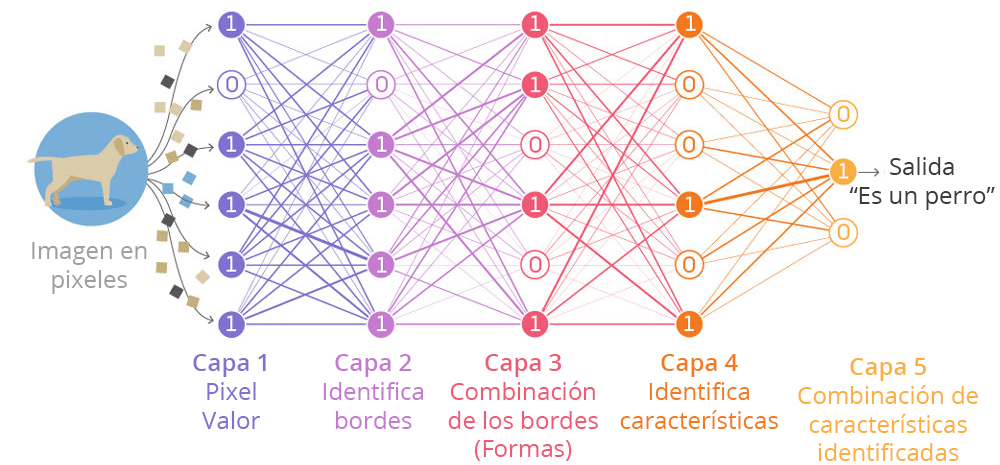
\includegraphics[width=\linewidth]{src/figures/deep_learning.png}
    \caption{Proceso de entrenamiento de una red deep learning \cite{deep_learning_img}}
    \label{fig:deep_learning_img}
\end{figure}

Entre los tipos de modelos de deep learning se encuentran 6 principales,
los cuales se explican de manera breve a excepción de las redes
neuronales convolucionales, las cuales son el enfoque principal del
presente trabajo de investigación.

\begin{itemize}
    \item \textbf{Redes Neuronales Convolucionales (CNN)}:
     utilizadas principalmente en el procesamiento de imágenes y 
     visión por computadora, conocidas por su capacidad para 
     capturar características espaciales.
    \item \textbf{Redes Neuronales Recurrentes (RNN)}: 
    diseñadas para trabajar con datos secuenciales, 
    como series temporales o lenguaje natural.
    \item \textbf{Redes Generativas Adversarias (GAN)}:
     compuestas de dos redes que compiten entre sí para generar datos
      sintéticos que se asemejan a datos reales, ampliamente utilizadas
       en generación de imágenes y contenido.
    \item \textbf{Autoencoders}: 
    redes que aprenden una representación comprimida de los datos
     de entrada y son útiles en tareas de reducción de dimensionalidad
      y compresión.
    \item \textbf{Modelos de difusión}: 
    Son modelos generativos entrenados con difusión directa e inversa
    para adicionar y eliminar ruido de las imágenes. estos modelos 
    generan datos en base a los datos de entrenamiento y añaden ruido 
    a los datos generados para aprender un proceso de eliminación de ruido.
    \item \textbf{Modelos de transformadores}: 
    Estos modelos usan una estructura de codificador y decodificador 
    para procesar texto. El codificador transforma el texto no procesado
    a representaciones llamadas incrustaciones, Después de esto,
    el decodificador usa esas incrustaciones resultantes 
    junto con palabras generadas previamente para generar texto que
    prediga la siguiente palabra en una oración de manera secuencial.
    \cite{ibm_deep_learning}
\end{itemize}

\subsection{Redes Neuronales Convolucionales}
Las redes neuronales convolucionales (CNN) son un tipo de red neuronal
que se utiliza principalmente en el procesamiento de imágenes y visión, 
aunque también son usadas en voz o audio. Estas redes neuronales se 
consituyen de varias capas las cuales pueden pertenecer a tres tipos:
capa convolucional, capa de agrupación y capa completamente conectada.
Para entender el funcionamiento de las redes neuronales convolucionales,
es necesario comprender el porque una imagen puede ser clasificada en
diferentes categorias; esto se debe a que las imagenes estan compuestas
por pixeles, los cuales son los elementos basicos de una imagen. Cada
pixel tiene un valor de intensidad que puede variar entre 0 y 255,
donde 0 representa el menor nivel de intensidad y 255 el mayor nivel
de intensidad.

\begin{figure}[ht!]
    \centering
    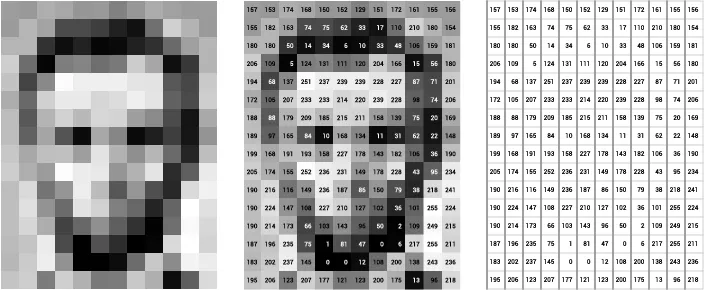
\includegraphics[width=\linewidth]{src/figures/grayscale_image.png}
    \caption{Imagen en escala de grises junto con sus valores por píxel \cite{grayscale_values}}
    \label{fig:grayscale_image}
\end{figure}

\newpage
Por otra parte, las imagenes pueden tener más de un canal
de color, como RGB (Red, Green, Blue), en este caso, cada canal de color
es una matriz de pixeles que representa un color en particular.

\begin{figure}[ht!]
    \centering
    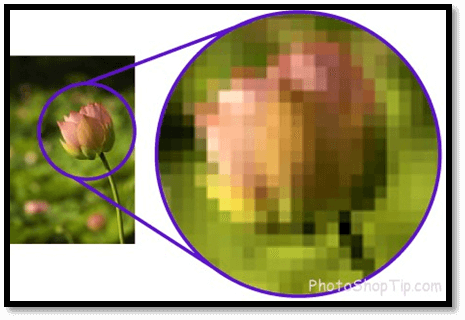
\includegraphics[width=\linewidth]{src/figures/pixels_in_image.png}
    \caption{Píxeles en una imagen \cite{pixels_in_image}}
    \label{fig:pixels_in_image}
\end{figure}

En adición, algunos conceptos básicos son definidos para asegurar la 
correcta comprensión de las redes neuronales convolucionales:

\begin{itemize}
    \item \textbf{Neurona}:
    Es la unidad básica de una red neuronal, la cual recibe una entrada
    y produce una salida al realizar una suma ponderada de sus conexiones
    a la que se le aplica una función de activación.
    \item \textbf{Función de activación}:
    Es una función matemática que se aplica a la salida de una neurona
    para determinar si esta se activa o no. Algunas de las funciones
    de activación más comunes son la función sigmoide, la función ReLU
    y la función tangente hiperbólica.
    \item \textbf{Capa de entrada}:
    Es la capa que recibe los datos de entrada, en esta, cada neurona
    corresponde a una de las características de entrada, como los pixeles
    de una imagen.
    Por ejemplo, si se tiene una imagen de 32x32 pixeles, la capa de
    entrada tendrá 1024 neuronas.
    \item \textbf{Capa oculta}:
    Son las posibles capas entre la capa de entrada y la capa de salida,
    las salidas de las neuronas de una capa oculta se convierten en las
    entradas de la siguiente capa.
    \item \textbf{Capa de salida}:
    Es la capa que produce la salida final de la red neuronal, en el caso
    de una red de clasificación, la capa de salida tendrá tantas neuronas
    como clases se desean clasificar.\cite{medium_cnn}
\end{itemize}


En cuanto a las funciones de activación, se explica el funcionamiento de 
cada una de ellas:

\begin{itemize}
    \item \textbf{Función Sigmoide}: 
    En algunos ejemplos es usada pero no es habitual, la función sigmoide
    se utiliza en la capa de salida de una red neuronal para problemas
    de clasificación binaria, ya que su salida se encuentra entre 0 y 1.
    Esto permite interpretar la salida como una probabilidad de pertenencia 
    a una clase específica. 
    Sin embargo, su uso ha disminuido en favor de otras funciones de activación,
     como ReLU, debido a problemas como el "desvanecimiento del gradiente" 
     y la saturación en valores extremos. A pesar de esto, la sigmoide sigue 
     siendo fundamental para entender cómo las redes neuronales pueden modelar
      relaciones no lineales y aprender patrones complejos \cite{sigmoid}.
    \begin{equation}
        f(x) = \frac{1}{1 + e^{-x}}
    \end{equation}

    \begin{figure}[H]
        \centering
        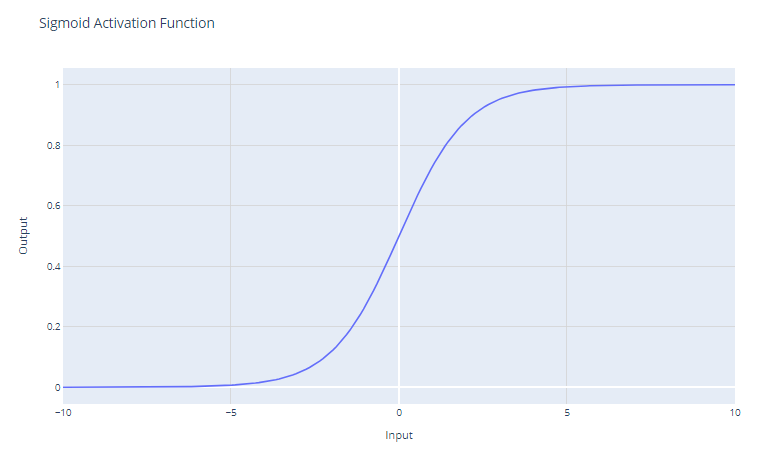
\includegraphics[width=\linewidth]{src/figures/sigmoid.png}
        \caption{Función Sigmoide \cite{sigmoid_graph}}
    \end{figure}

    \item \textbf{Función Tangente Hiperbólica}:
    La función de activación \textbf{tanh} (tangente hiperbólica) transforma valores 
    reales en un rango de -1 a 1, siendo útil en redes neuronales para centrar los 
    datos alrededor de cero. Su derivada es \(1 - \text{tanh}^2(x)\), lo que puede 
    causar saturación y desvanecimiento del gradiente en redes profundas. 
    A pesar de esto, es popular en capas ocultas por su capacidad de manejar tanto valores positivos 
    como negativos. \cite{activation_functions}

    \begin{equation}
        f(x) = \frac{e^{x} - e^{-x}}{e^{x} + e^{-x}}
    \end{equation}

    \begin{figure}[H]
        \centering
        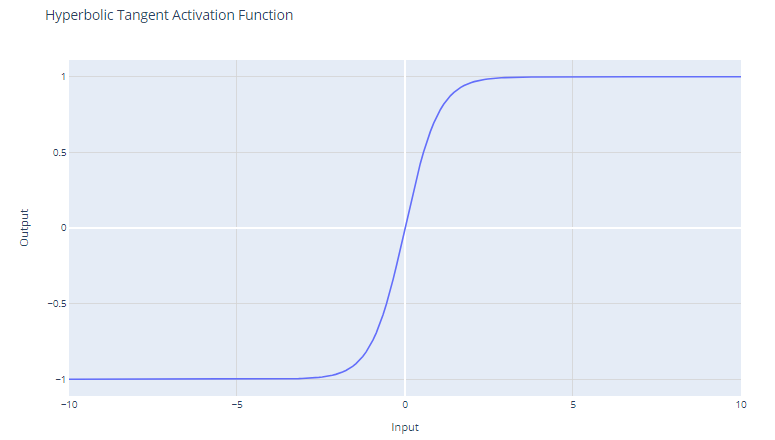
\includegraphics[width=\linewidth]{src/figures/tanh.png}
        \caption{Función Tangente Hiperbólica \cite{tanh_graph}}
    \end{figure}

    \item \textbf{Función ReLU (Rectified Linear Unit)}:
    La función de activación ReLU (Unidad Lineal Rectificada) es ampliamente utilizada 
    en redes neuronales por su simplicidad y efectividad, definida como:

        \[
        f(x) = \max(0, x)
        \]

    ReLU retorna 0 para valores negativos y el valor original para valores positivos, 
    permitiendo que el gradiente pase sin alteración en la retropropagación y evitando 
    el problema del gradiente que se desvanece. Aunque es lineal para entradas positivas, 
    su no linealidad en \( x = 0 \) le permite captar patrones complejos. 
    Además, su bajo costo computacional y tendencia a activaciones esparsas 
    favorecen la eficiencia en redes profundas. \cite{activation_functions}

    \begin{figure}[H]
        \centering
        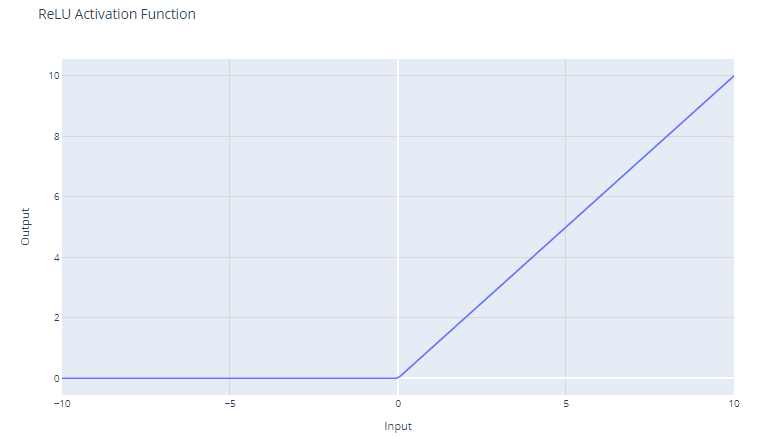
\includegraphics[width=\linewidth]{src/figures/relu.png}
        \caption{Función ReLU \cite{relu_graph}}
    \end{figure}

    \item \textbf{Función Softmax}:
    La función de activación Softmax es útil para clasificación multiclase, 
    convirtiendo un vector de entradas \( x_1, x_2, \dots, x_C \) en una distribución de probabilidad:

    \[
    f(x_i) = \frac{e^{x_i}}{\sum_{j} e^{x_j}}
    \]

    Cada salida representa la probabilidad de pertenencia a una clase, sumando a uno. 
    Softmax amplifica las diferencias entre entradas, haciendo que el valor más alto domine, 
    y se emplea comúnmente en la capa final de redes neuronales para tareas de clasificación 
    multiclase, proporcionando interpretaciones probabilísticas de confianza en las predicciones.
    \cite{activation_functions}

    \begin{figure}[H]
        \centering
        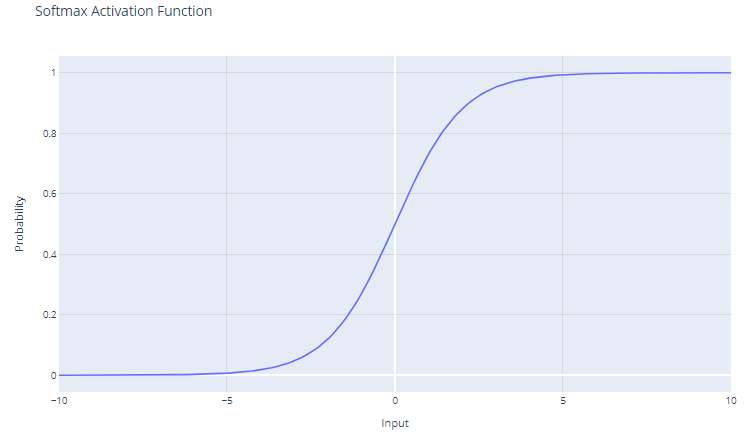
\includegraphics[width=\linewidth]{src/figures/softmax.png}
        \caption{Función Softmax \cite{softmax_graph}}
    \end{figure}
    
\end{itemize}

Una vez que se tienen claros los conceptos básicos, en las CNN se 
tienen tres tipos de capas, las cuales fueron descritas anteriormente:

\subsubsection{Capa Convolucional}

Esta capa es la parte fundamental de las redes neuronales convolucionales,
en esta capa son necesarios los elementos normales como las entradas, lo 
que la hace diferente es su necesidad de un filtro y un mapa de 
características. El filtro, también conocido como Kernel, es una matriz
de pesos (numeros) que se aplica a la imagen de entrada, este kernel se
desliza través de cada píxel para extraer características tales 
como bordes, texturas, formas, entre otros. La imagen resultante se
compone de un producto punto entre el kernel y cada pixel de la imagen. 
Los Kernel pueden ser de diferentes tamaños y pueden ser predefinidos 
o aprendidos durante el entrenamiento de la red.
Un ejemplo de un Kernel habitualmente usado es el Kernel de Sobel, el
cual se utiliza para detectar bordes en una imagen.

\begin{figure}[ht!]
    \centering
    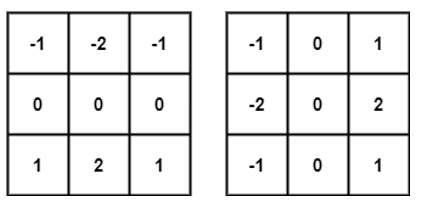
\includegraphics[width=\linewidth]{src/figures/sobel_kernel.png}
    \caption{Kernel de Sobel Horizontal y Vertical \cite{sobel_kernel}}
    \label{fig:sobel_kernel}
\end{figure}

Otro de los aspectos clave es que el tamaño del resultado se ve 
afectado por los siguientes hiperparametros:

\begin{itemize}
    \item \textbf{Cantidad de filtros}:
    La cantidad de filtros afecta a la profundidad de la salida, 
    esto porque cada filtro produce un mapa de características. 
    Por ejemplo, si se tienen 6 filtros y se recibe una imagen con 
    un solo canal de color, la salida tendrá 6 canales de color, pero
    si se recibe una imagen con 3 canales de color como RGB, la salida
    tendrá 18 canales de color (18 mapas de características).
    \item \textbf{Stride}:
    Es el número de píxeles que se desplaza el filtro en cada paso.
    \item \textbf{Padding}:
    Es la cantidad de píxeles que se añaden alrededor de la imagen, 
    generalmente se usa cuando el filtro es más grande que la imagen, 
    el borde que se le añade a la imagen es con valores de 0.
    \item \textbf{Tamaño del filtro}:
    Es el tamaño del filtro que se desliza sobre la imagen, generalmente
    se usan filtros de 3x3 o 5x5.
\end{itemize}

El calculo final para el tamaño que tendra un mapa de características
despues de aplicar un filtro a una imagen es el siguiente:

\begin{equation}
    \text{Salida} = \frac{N - K + 2P}{S} + 1
\end{equation}

Donde:
\begin{itemize}
    \item \textbf{N:} Tamaño de la imagen de entrada.
    \item \textbf{K:} Tamaño del filtro.
    \item \textbf{P:} Padding.
    \item \textbf{S:} Stride.
    \item \textbf{Salida:} Tamaño de la imagen de salida.
\end{itemize}

\newpage

Un ejemplo claro del calculo relizado con un filtro de 3x3 y una 
imagen de 5x5 es el siguiente:

\begin{figure}[ht!]
    \centering
    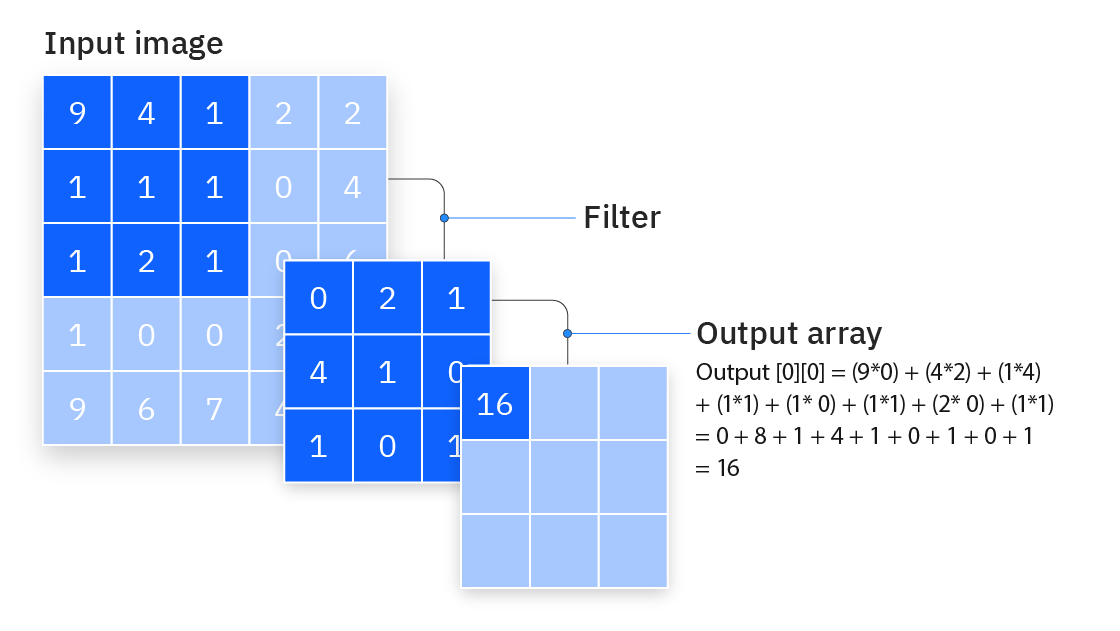
\includegraphics[width=\linewidth]{src/figures/kernel_calculation.png}
    \caption{Capa convolucional aplicada a una imagen \cite{kernel_calculation}}
    \label{fig:kernel_calculation}
\end{figure}

Cabe aclarar que puede haber más de una capa convolucional en una red,
esto convierte la estructura de la CNN en jerárquica, donde cada capa
que sigue a la anterior, aprende características más complejas.

\subsubsection{Capa de Agrupación}
La capa de agrupación (Pooling) es una capa que se utiliza para reducir
las dimensiones (Ancho y Alto) de la imagen, para disminuir el número
de parámetros y el costo computacional. La agrupacion aplica una función
de agregación a un conjunto de píxeles, como el promedio o el máximo; 
Esta capa aunque pierde información, ayuda a mejorar la generalización
de la red y su eficiencia. La capa de agrupacion puede ser de los 
siguientes tipos \cite{medium_pooling}:

\begin{itemize}
    \item \textbf{Max Pooling}:
    Se selecciona el valor máximo de un conjunto de píxeles, por lo tanto
    la salida despues de la capa de max pooling sera el mapa de características
    con los valores más altos.

    \begin{figure}[htbp]
        \centering
        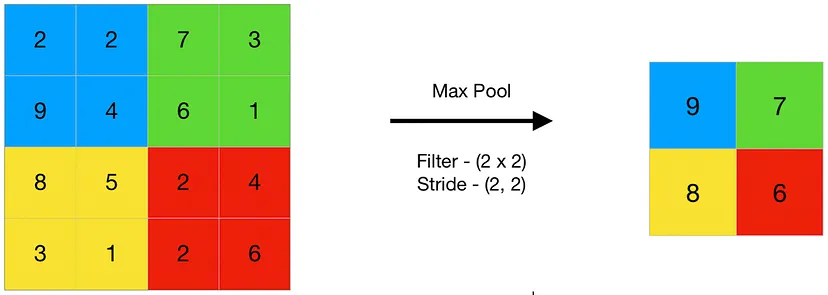
\includegraphics[width=0.8\linewidth]{src/figures/max_pooling.png}
        \caption{Max Pooling aplicado a un mapa de características \cite{max_pooling}}
        \label{fig:max_pooling}
    \end{figure}

    \item \textbf{Average Pooling}:
    Se calcula el promedio de un conjunto de píxeles en el mapa de características,
    por lo tanto la salida despues de la capa de average pooling sera el mapa de
    características con los valores promedio.

    \begin{figure}[htbp]
        \centering
        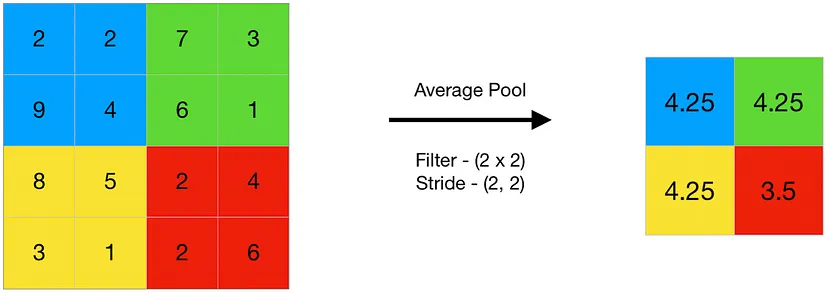
\includegraphics[width=0.8\linewidth]{src/figures/average_pooling.png}
        \caption{Average Pooling aplicado a un mapa de características \cite{average_pooling}}
        \label{fig:average_pooling}
    \end{figure}
\end{itemize}

Además de estos tipos, tambien hay agrupamiento global, el cual calcula
el promedio o el máximo de cada canal de características, en lugar de
hacerlo por regiones; Esto da como salida un solo valor por canal de
características.

\subsubsection{Capa Completamente Conectada}
Normalmente, suele haber una capa entre la capa de agrupación y la capa
completamente conectada, esta capa se conoce como capa de aplanamiento
(Flatten), la cual convierte la matriz de características en un vector
unidimensional, para que pueda ser procesado por la capa completamente
conectada.

\begin{figure}[htbp]
    \centering
    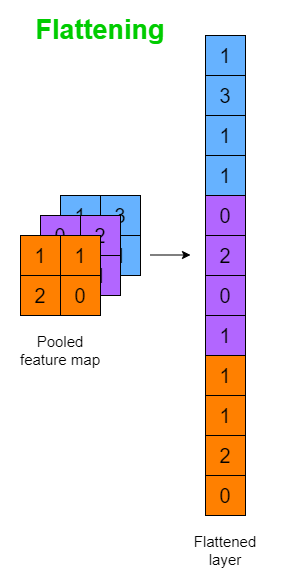
\includegraphics[width=0.45\linewidth]{src/figures/flatten.png}
    \caption{Capa de aplanamiento aplicada a tres mapas de características \cite{capa_aplanada}}
    \label{fig:flatten}
\end{figure}

Por último, la capas capas completamente conectadas son las capas
de una RNA tradicional, donde cada neurona de la capa está conectada
con todas las neuronas de la capa anterior. Estas capas se utilizan
para clasificar las características extraídas por las capas convolucionales
y de agrupación. La capa completamente conectada se encarga de realizar
la clasificación final de la red, en donde se obtiene la probabilidad
de que una imagen pertenezca a una clase en particular mediante la 
función de activación softmax.

\begin{figure}[htbp]
    \centering
    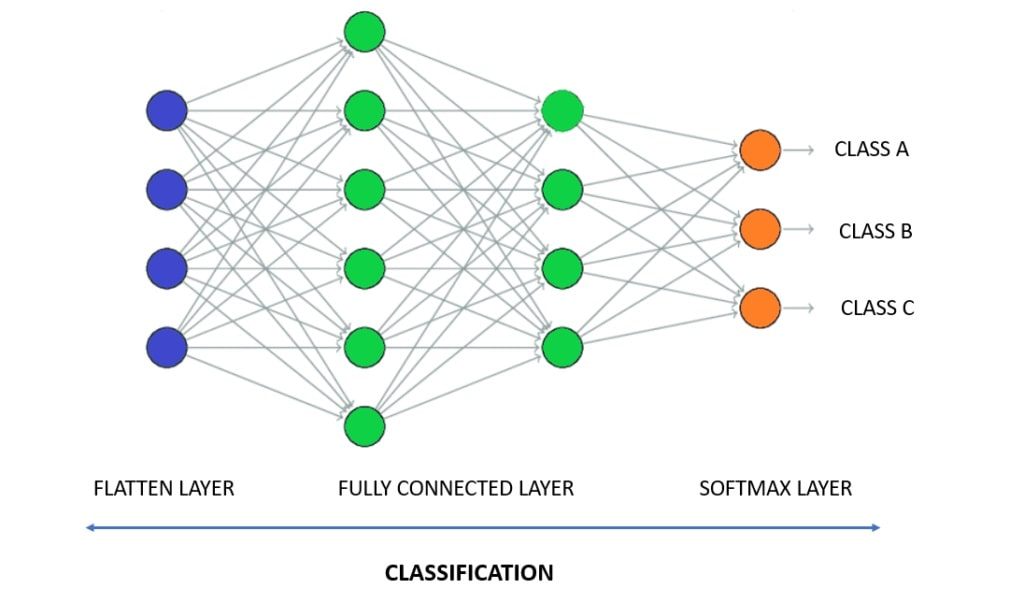
\includegraphics[width=0.9\linewidth]{src/figures/fully_connected_layer.png}
    \caption{Capa completamente conectada \cite{capa_conectada}}
    \label{fig:fully_connected}
\end{figure}


\subsection{LeNet}

\subsubsection{Historia}

La historia de LeNet refleja un progreso innovador en el desarrollo 
de redes neuronales convolucionales aplicadas a la identificación de 
patrones visuales. En 1988, Yann LeCun se unió al Departamento de 
Investigación de Sistemas Adaptativos en AT\&T Bell Labs, dirigido 
por Lawrence D. Jackel. Desde entonces, LeCun y su equipo comenzaron 
a trabajar en modelos que pudieran reconocer caracteres manuscritos 
de manera eficiente, en particular códigos postales.

En 1989, publicaron la primera versión de una red neural convolucional
 (LeNet-1) diseñada específicamente para leer dígitos manuscritos. 
 Esta versión utilizaba núcleos de convolución fijos y se entrenaba
 mediante el algoritmo de retropropagación, lo cual era una innovación 
 importante en el campo. Este primer modelo mostró que la combinación 
 de redes convolucionales y retropropagación podía aprender a 
 generalizar características visuales relevantes con una alta precisión,
  incluso en tareas complejas como el reconocimiento de dígitos 
  manuscritos proporcionados por el Servicio Postal de los Estados 
  Unidos. En este año también, LeCun demostró que la restricción 
  del número de parámetros libres mejoraba significativamente la 
  capacidad de generalización del modelo.

En 1990, se publicaron más investigaciones sobre la aplicación de redes 
de retropropagación para reconocimiento de caracteres, logrando un 
margen de error bajo en la identificación de números en imágenes, 
con una tasa de rechazo controlada. Estos resultados alentaron 
investigaciones continuas, y en 1994, LeCun y su equipo desarrollaron 
la base de datos MNIST, diseñada como un estándar para evaluar redes 
de reconocimiento de dígitos. LeNet-4 se entrenó para abordar el tamaño 
y la complejidad de esta base de datos.

El esfuerzo culminó en 1995 con el desarrollo de LeNet-5, 
una arquitectura más avanzada que integraba métodos adicionales 
para mejorar la precisión en la clasificación de caracteres manuscritos. 
Este modelo no solo superó otros métodos en pruebas de referencia, 
sino que también fue aplicado en sistemas de lectura automática de 
millones de cheques bancarios al día. En 1998, LeCun y su equipo 
presentaron estos avances como ejemplos de aplicaciones prácticas en el 
reconocimiento de caracteres manuscritos.

Aunque las redes neuronales modernas han evolucionado significativamente 
desde LeNet, esta serie de modelos sentó las bases para el diseño de 
arquitecturas convolucionales complejas, marcando un hito en la historia 
de la inteligencia artificial y el aprendizaje profundo \cite{lenet_history_geeks} \cite{lenet_neha}.

\subsubsection{versiones}

\begin{itemize}
    \item \textbf{LeNet-1}: 
    LeNet-1 fue uno de los primeros modelos de redes neuronales 
    convolucionales diseñado por Yann LeCun y su equipo. 
    La arquitectura estaba enfocada en reconocer dígitos manuscritos 
    y se basaba en la aplicación de capas de convolución y capas de 
    subsampling o pooling. Los detalles de su arquitectura son los 
    siguientes:

    \begin{figure}[htbp]
        \centering
        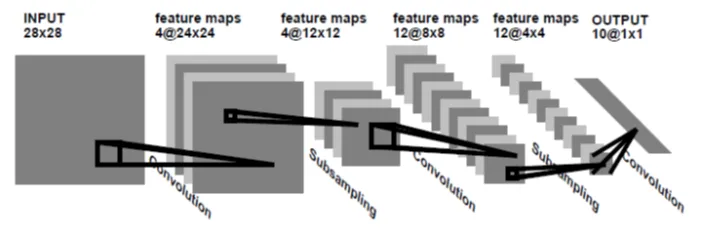
\includegraphics[width=\linewidth]{src/figures/lenet_1.png}
        \caption{Arquitectura de LeNet-1 \cite{Lenet_1}}
        \label{fig:lenet-1}
    \end{figure}

    \textbf{Entrada}: Imagen de 28x28 píxeles en escala de grises.  
    \textbf{Capa de convolución 1}: genera cuatro mapas de características
    de 24x24 píxeles mediante la convolución con kernels predefinidos de 5x5 píxeles.

    \textbf{Capa Average Pooling 1}: reduce la dimensión de los mapas de características
    a 12x12 píxeles usando una ventana de 2x2 píxeles para calcular el promedio.

    \textbf{Capa de convolución 2}: produce 12 mapas de características 
    de 8x8 píxeles mediante la convolución con kernels de 5x5 píxeles.

    \textbf{Capa Average Pooling 2}: reduce la dimensión de los mapas de 
    características a 4x4 píxeles usando una ventana de 2x2 píxeles 
    para calcular el promedio.

    \textbf{Capa de Salida}: capa completamente conectada con 10 neuronas
    para clasificar los dígitos del 0 al 9.

    \item \textbf{LeNet-4}:
    
    LeNet-4 es una versión mejorada de LeNet-1, diseñada para manejar 
    imágenes de entrada ligeramente más grandes y con más capacidad 
    de aprendizaje. La arquitectura de LeNet-4 tiene los siguientes 
    componentes:

    \begin{figure}[htbp]
        \centering
        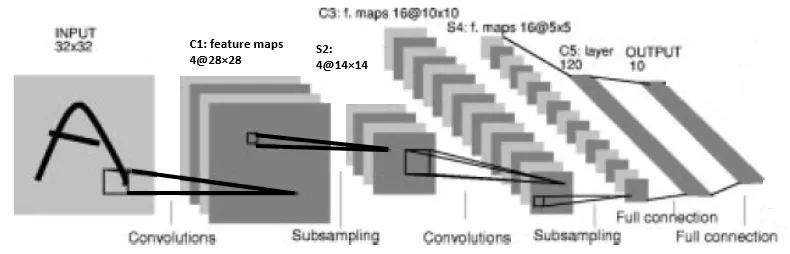
\includegraphics[width=\linewidth]{src/figures/lenet_4.png}
        \caption{Arquitectura de LeNet-4 \cite{Lenet_4}}
        \label{fig:lenet-4}
    \end{figure}

    \textbf{Entrada}: Imagen de 32x32 píxeles en escala de grises.

    \textbf{Capa de convolución 1}: genera cuatro mapas de 
    características de 28x28 píxeles mediante la convolución con
    kernels de 5x5 píxeles.

    \textbf{Capa Average Pooling 1}: reduce la dimensión de los mapas
    de características a 14x14 píxeles usando una ventana de 2x2 píxeles
    para calcular el promedio.

    \textbf{Capa de convolución 2}: produce 16 mapas de características
    de 10x10 píxeles mediante la convolución con kernels de 5x5 píxeles.

    \textbf{Capa Average Pooling 2}: reduce la dimensión de los mapas
    de características a 5x5 píxeles usando una ventana de 2x2 píxeles
    para calcular el promedio. 

    \textbf{Flatten Layer}: convierte los mapas de características en
    un vector unidimensional.

    \textbf{Capa completamente conectada 1}: 120 neuronas con función
    de activación sigmoidal o tangente hiperbólica.

    \textbf{Capa de Salida}: 10 neuronas con función
    de activación softmax para clasificar los dígitos del 0 al 9.

    \item \textbf{LeNet-5}:

    LeNet-5 es la versión más popular de la arquitectura LeNet, 
    introducida en 1995. Es similar a LeNet-4, pero incluye algunos 
    ajustes adicionales en la cantidad de neuronas y conexiones. 
    Su estructura es la siguiente:

    \begin{figure}[ht!]
        \centering
        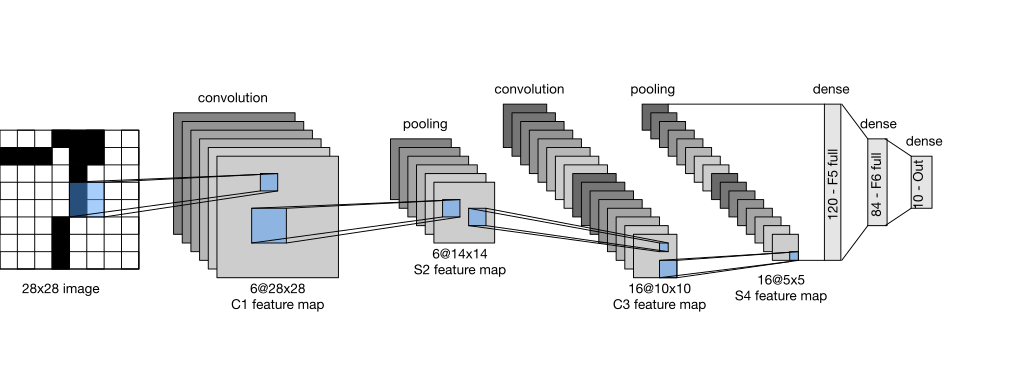
\includegraphics[width=\linewidth]{src/figures/lenet_5.png}
        \caption{Arquitectura de LeNet-5 \cite{Lenet_5}}
        \label{fig:lenet-5}
    \end{figure}

    \textbf{Entrada}: Imagen de 32x32 píxeles en escala de grises.

    \textbf{Capa de convolución 1}: genera seis mapas de características
    de 28x28 píxeles mediante la convolución con kernels de 5x5 píxeles.

    \textbf{Capa Average Pooling 1}: reduce la dimensión de los mapas
    de características a 14x14 píxeles usando una ventana de 2x2 píxeles
    para calcular el promedio.

    \textbf{Capa de convolución 2}: produce 16 mapas de características
    de 10x10 píxeles mediante la convolución con kernels de 5x5 píxeles.

    \textbf{Capa Average Pooling 2}: reduce la dimensión de los mapas
    de características a 5x5 píxeles usando una ventana de 2x2 píxeles
    para calcular el promedio.

    \textbf{Flatten Layer}: convierte los mapas de características en
    un vector unidimensional.

    \textbf{Capa completamente conectada 1}: 120 neuronas con función
    de activación sigmoidal o tangente hiperbólica.

    \textbf{Capa completamente conectada 2}: 84 neuronas con función
    de activación sigmoidal o tangente hiperbólica.

    \textbf{Capa de Salida}: 10 neuronas con función
    de activación softmax para clasificar los dígitos del 0 al 9.

    \space

    \item \textbf{Boosted LeNet-4}:
    
    \begin{figure}[htbp]
        \centering
        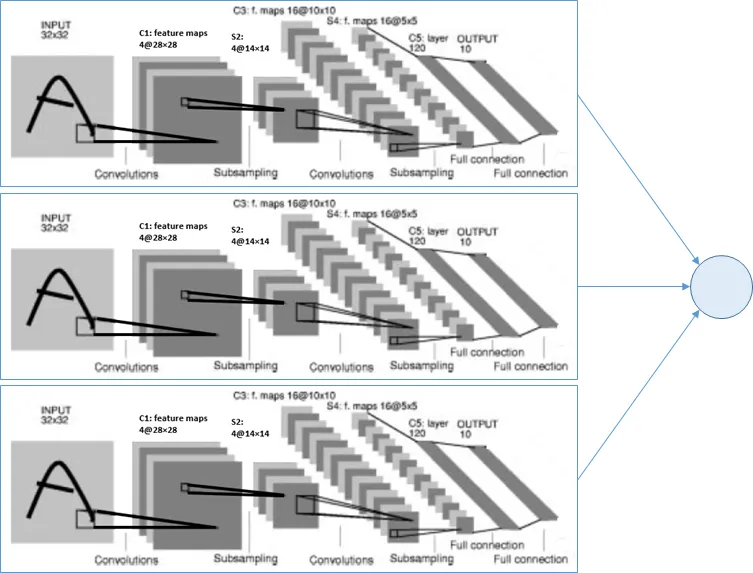
\includegraphics[width=\linewidth]{src/figures/lenet_4_boosted.png}
        \caption{Arquitectura de Boosted LeNet-4 \cite{LeNet_4_boosted}}
        \label{fig:boosted_lenet_4}
    \end{figure}

    En una versión mejorada llamada Boosted LeNet-4, se implementó 
    una técnica de combinación de múltiples redes para aumentar 
    la precisión de LeNet-4. Esta técnica de boosting combinaba los 
    resultados de tres redes LeNet-4; se sumaban las salidas y el 
    valor más alto era la clase predicha. Además, si una red obtenía 
    una salida con alta confianza, las demás redes no se usaban. 
    Con esta modificación, Boosted LeNet-4 redujo la tasa de error 
    a 0.7\%, mejorando incluso a LeNet-5.

\end{itemize}

\subsubsection{Aplicaciones}

La red neuronal convolucional LeNet ha demostrado ser una 
arquitectura fundamental que trasciende su propósito inicial 
de reconocimiento de dígitos manuscritos tal como se ve presente
en el desarrolló realizado por Yann LeCun en su articulo sobre LeNet,
en aquella ocación la implementación logro una precisión de 
clasificación de aproximadamente el 99,2\%, aunque el documento 
original es largo y trata varios temas, cabe recalcar la comparación
con modelos de clasificación del momento dando un porcentaje de 
error bastante más bajo con respecto a los otros modelos, entre los
modelos contra los cuales fue comparado están: K-NN, Support Vector
Machine y diferentes combinaciones de capas de neuronas. 

\begin{figure}[htbp]
    \centering
    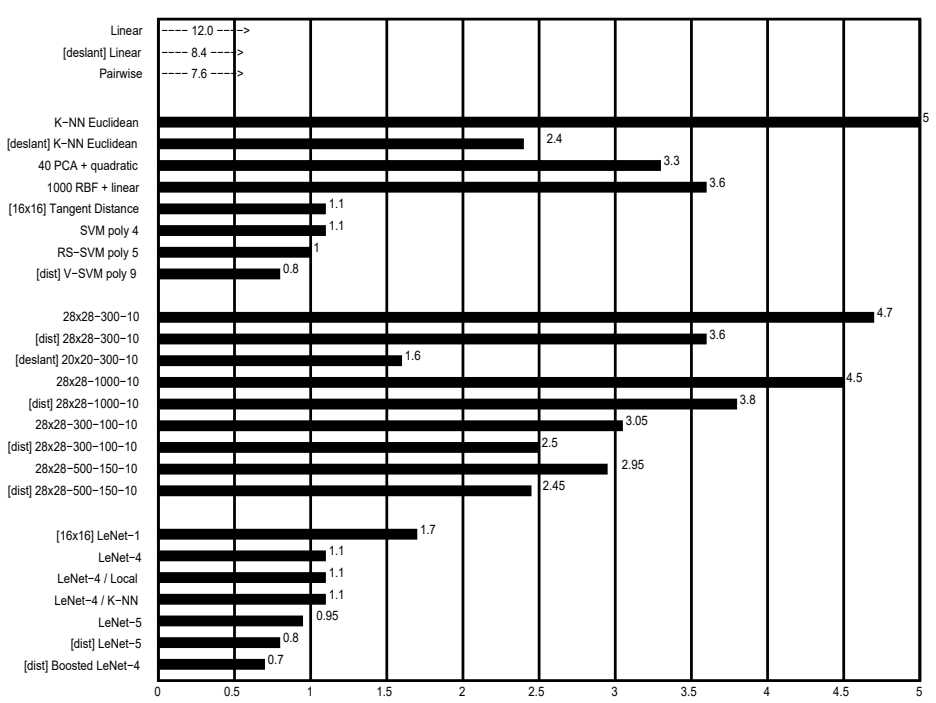
\includegraphics[width=\linewidth]{src/figures/lenet_comparison.png}
    \caption{Comparación de LeNet con otros modelos de clasificación \cite{lecun_comparison_image}}
    \label{fig:lenet_comparison}
\end{figure}

Sus aplicaciones se han diversificado significativamente en diversos 
campos tecnológicos y científicos. En el sector de procesamiento documental, 
 esta arquitectura facilita la automatización de tareas de gestión y 
 clasificación de documentos, mientras que en el ámbito médico 
 contribuye al análisis de imágenes diagnósticas para la identificación 
 de anomalías, un claro ejemplo de esto es el articulo llamado 
 A Modified LeNet CNN for Breast Cancer Diagnosis in Ultrasound Images 
 \cite{lenet_medical} donde se utiliza una versión modificada de LeNet
    para la detección de cancer de mama en imagenes de ultrasonido, 
 este modelo se planteó como un clasificador de tumores benignos y
    malignos, obteniendo una precisión del 89.91\% en el reconocimiento
    de imagen. El sistema también ha revolucionado los procesos de 
 autenticación biométrica mediante el análisis de firmas y huellas 
 dactilares, fortaleciendo los protocolos de seguridad. 
 En el contexto del análisis de video en tiempo real, los principios 
 de LeNet han sido instrumentales para el desarrollo de sistemas de 
 vigilancia y reconocimiento facial, En este campo, se tiene como 
 ejemplo práctico el artículo online publicado por Andrii Gozhulovskyi
 llamado Classification of Traffic Signs with LeNet-5 CNN
 \cite{lenet_traffic_sings} donde se usan los datos de las señales de 
 trafico alemanas para entrenar una red LeNet-5 que permita 
 clasificarlas, este articulo comprende un tutorial paso a paso de 
 como implementar la red junto con sus datos, evaluacion y graficación
 de resultados y métricas. Adicionalmente, su implementación 
 en el reconocimiento de caracteres manuscritos ha facilitado la
  digitalización de documentos históricos y el procesamiento 
  automatizado de formularios en diversos sectores, incluyendo servicios
   postales y bancarios. La versatilidad de esta arquitectura ha 
   permitido su adaptación para la clasificación de objetos en entornos 
   industriales y comerciales, demostrando su valor en sistemas de 
   control de calidad y gestión de inventarios 
   \cite{lenet_history_geeks}.

\subsubsection{Limitaciones}

Con respecto a las limitaciones de la red LeNet, se pueden mencionar
algunas de las siguientes:

\begin{itemize}
    \item \textbf{Capacidad de generalización}:
    Al ser una arquitectura relativamente simple, LeNet puede tener
    una limitacion para generalizar tareas complejas, esto debido a su
    pequeño tamaño y cantidad de capas.
    \item \textbf{Tamaño de entrada}:
    Se restringe su aplicabilidad a imagenes de tamaño fijo (32x32),
    lo cual es ineficaz para aplicaciones del mundo real donde 
    las imagenes varian en tamaño.
    \item \textbf{Falta de escalabilidad}:
    Puede ser un modelo que se queda corto en adaptaciones a 
    datos modernos y demandas de deep learning.\cite{lenet_neha}
\end{itemize}
\section{Metodología}
Esta sección describe la metodología utilizada para la implementación de la red neuronal convolucional LeNet-5. 
Se describen los pasos seguidos para la implementación de la red, la obtención de los datos, el preprocesamiento de los datos, 
la implementación de la red y la evaluación de la red.
Esta red LeNet se enfocó en la clasificación de números, con una funcionalidad en tiempo real
para la predicción de números capturados por cámara y fue implementada en Python con la librería TensorFlow.

\subsection{Obtención de los datos}
Los datos usados fueron obtenidos de la base de datos Housenumbers (SVHN) que contiene imágenes de números de casas.
La base de datos contiene 73257 imágenes de entrenamiento y 26032 imágenes de prueba, pero se usaron 
los 600,000 datos extra para el entrenamiento de la red, quedando un total de 673,257 imágenes de entrenamiento 
y 26032 imágenes de prueba. Esta base de datos contiene un formato de imágenes de 32x32 pixeles, con 3 canales de color 
y se escogió para la implementación de la red LeNet-5 principalmente para adecuarla a un entorno más realista.

Estos datos están disponibles en la pagina web de SVHN \cite{shvn_color} en donde se da el conjunto de datos en formato .mat, por este motivo, 
la lectura de los datos se uso con la librearía \texttt{spicy.io} la cual permite leer el formato .mat mediante la implementación
de las siguientes dos funciones:

\begin{lstlisting}
    def initialize_svhn_info():
    global train_images, train_labels, test_images, test_labels
    # Cargar los datos SVHN
    train_images, train_labels = load_svhn_data(get_resource_path('Data/train_32x32.mat'))
    test_images, test_labels = load_svhn_data(get_resource_path('Data/test_32x32.mat'))
    extra_images, extra_labels = load_svhn_data(get_resource_path('Data/extra_32x32.mat'))
    
    # Concatenar los conjuntos de entrenamiento y extra
    train_images = np.concatenate([train_images, extra_images], axis=0)
    train_labels = np.concatenate([train_labels, extra_labels], axis=0)

    # Convertir las etiquetas a formato categórico
    train_labels = to_categorical(train_labels)
    test_labels = to_categorical(test_labels)
\end{lstlisting}

\begin{lstlisting}
    def load_svhn_data(mat_file_path):
    # Cargar el archivo .mat
    svhn_data = scipy.io.loadmat(mat_file_path)
    images = svhn_data['X']  # Contiene las imágenes
    labels = svhn_data['y']  # Contiene las etiquetas

    # Cambiar la etiqueta 10 a 0 (en SVHN, 10 representa el dígito 0)
    labels[labels == 10] = 0

    # Convertir imágenes de (32, 32, 3, N) a (N, 32, 32, 3)
    images = np.moveaxis(images, -1, 0)
    
    # Convertir a escala de grises y normalizar
    images_gray = np.array([cv2.cvtColor(img, cv2.COLOR_RGB2GRAY) / 255.0 for img in images])

    return images_gray, labels
\end{lstlisting}

En las función llamada \textbf{\texttt{initialize\_svhn\_info}} se accede a las rutas tanto de los conjuntos de entrenamiento, pruebas
y los datos extras, todos los archivos se ubicaron en una carpeta llamada \textbf{Data}, para cargar los datos se usa la segunda función,
en donde mediante la función \textbf{\texttt{loadmat}} se carga el archivo en formato .mat pasandole una ruta especificada, una
vez se lee la información contenida en los archivo , se separan las imagenes y se guardan en una variable (X) y las etiquetas de 
las imagenes en otra variable (y), después de esto, se cambia la etiqueta \textbf{10} a \textbf{0} y se convierten a un formato
adecuado con la función \textbf{\texttt{moveaxis}} para cambiar la orientación de la matriz que representa la imagen a una valida
para la manipulación en la red LeNet. Una vez que el proceso se realiza, se combinan el conjunto de datos de entrenamiento y el 
extra en uno solo con la funcion de numpy para concatenar; Por otra parte, en la finalización del proceso se convierten las etiquetas
de indentificación en una etiqueta valida para Softmax, como ejemplo, para el número 1 se tendría una etiqueta de las siguiente manera:
[0,1,0,0,0,0,0,0,0,0] en donde 1 representaría que esa posición tiene un 100\% de probabilidad.

Algunos ejemplos de las imagenes de entrada son los siguientes:

\begin{figure}[htbp]
    \centering
    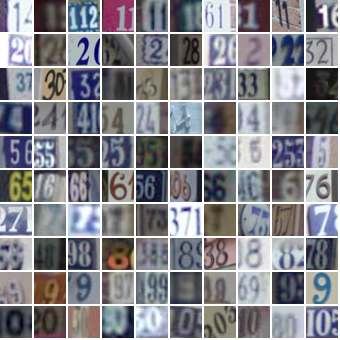
\includegraphics[width=\linewidth]{src/figures/shvn_color.png}
    \caption{Ejemplo de imagenes del conjunto de datos SHVN \cite{shvn_color}}
    \label{fig:shvn_color}
\end{figure}

\subsection{Preprocesamiento de los datos}
Para el preprocesamiento de los datos, se realizó una conversion a escala de grises de las imágenes y se normalizaron los datos,
esto se hizo por medio de la librearía OpenCV en Python con el siguiente código que se encuentra dentro de la anterior función
para el cargue de datos. 

\begin{lstlisting}
    np.array([cv2.cvtColor(img, cv2.COLOR_RGB2GRAY) / 255.0 for img in images])
\end{lstlisting}

este código permite hacer una matriz con la cantidad de imagenes y en esa matriz se agregan los datos pasados a escala de grises con
la función \textbf{\texttt{cvtColor}} especificando la imagen y el formato nuevo de color en los parametros, por último, se usa 
la division entre 255 para cada imagen y así normalizarla.

\newpage

\begin{figure}[H]
    \centering
    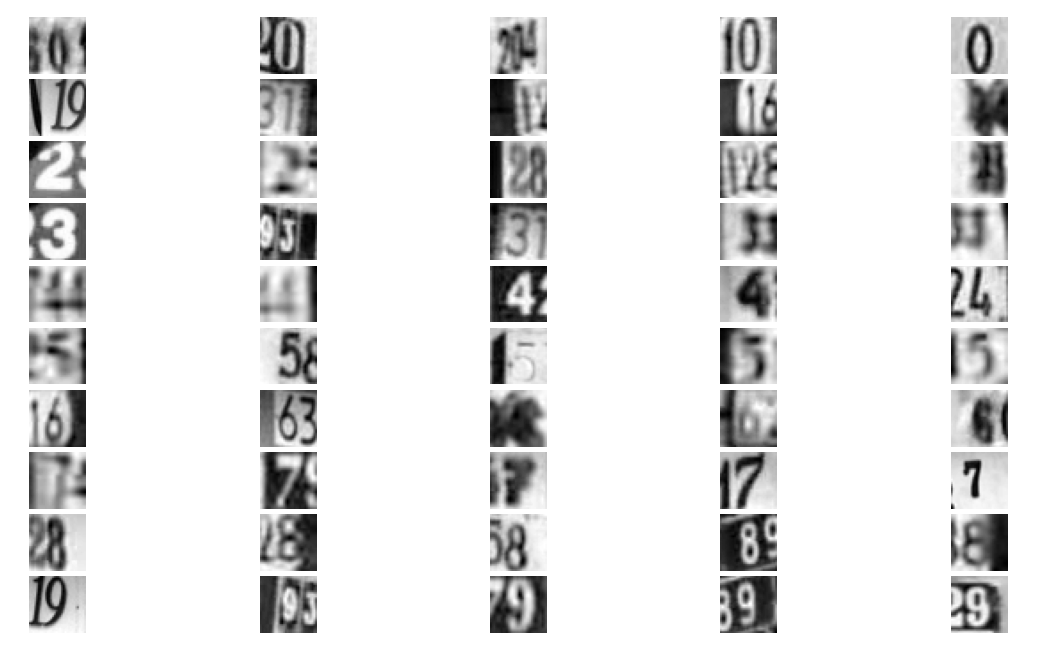
\includegraphics[width=\linewidth]{src/figures/shvn_gray.png}
    \caption{Ejemplo de imagenes del conjunto de datos SHVN en escala de grises}
    \label{fig:shvn_gray}
\end{figure}

\subsection{Implementación de la red LeNet-5}

Una vez se ha realizado el tratamiento de las imágenes se debe inicializar la red LeNet, para la construcción de esta, se usaron
las funcionalidades de \textbf{Keras} que se encuentran en la librearía de \textbf{TensorFlow}. 

Para implementar la arquitectura en código python se requiere de las siguientes lineas de código:

\begin{lstlisting}
    # Definir la arquitectura de LeNet-5
    model = models.Sequential()
    model.add(keras.Input(shape=(32, 32, 1)))
    model.add(layers.Conv2D(6, (5, 5), activation='relu'))
    model.add(layers.AveragePooling2D(pool_size=(2, 2)))
    model.add(layers.Conv2D(16, (5, 5), activation='relu'))
    model.add(layers.AveragePooling2D(pool_size=(2, 2)))
    model.add(layers.Flatten())
    model.add(layers.Dense(120, activation='relu'))
    model.add(layers.Dense(84, activation='relu'))
    model.add(layers.Dense(10, activation='softmax'))
    # Compilar el modelo
    model.compile(optimizer='adam', loss='categorical_crossentropy', metrics=['accuracy'])
\end{lstlisting}

Aquí hay varias funciones clave:

\begin{itemize}
    \item \textbf{\texttt{models.Sequential()}}: Crea una instancia del modelo secuencial de Keras. 
    Un modelo secuencial es una pila de capas donde la salida de una capa se convierte en la entrada de la siguiente capa.  
    \item \textbf{\texttt{add(layer):}} Agrega una capa al modelo.
    \item \textbf{\texttt{keras.Input(shape=(32, 32, 1))}}: Define la forma de entrada de la red. 
    La capa de entrada especifica la forma de los datos de entrada que alimentarán al modelo. 
    En este caso, los datos de entrada tienen una forma de (32, 32, 1), lo que significa que cada imagen 
    tiene una dimensión de 32x32 píxeles y un solo canal (escala de grises).
    \item \textbf{\texttt{layers.Conv2D(6, (5, 5), activation='relu')}}: Agrega una capa convolucional 2D al modelo.
    La capa de convolución aplicará 6 filtros de 5x5 píxeles a las imágenes de entrada. 
    Cada filtro aprenderá a detectar características particulares de las imágenes. 
    La función de activación utilizada es ReLU (Rectified Linear Unit), que ayuda a introducir no linealidad en el modelo.
    \item \textbf{\texttt{layers.AveragePooling2D(pool\_size=(2, 2))}}: Agrega una capa de agrupación promedio 2D al modelo.
    \item \textbf{\texttt{layers.Conv2D(16, (5, 5), activation='relu')}}: Agrega otra capa convolucional 2D al modelo.
    Esta capa aplicará 16 filtros de 5x5 píxeles a las imágenes de entrada.
    \item \textbf{\texttt{layers.Flatten()}}: Agrega una capa de aplanado al modelo.
    \item \textbf{\texttt{layers.Dense(120, activation='relu')}}: Agrega una capa densa al modelo que cuenta con 120 neuronas
    y utiliza la función de activación ReLU.
    \item \textbf{\texttt{layers.Dense(84, activation='relu')}}: Agrega otra capa densa al modelo que cuenta con 84 neuronas
    y utiliza la función de activación ReLU.
    \item \textbf{\texttt{layers.Dense(10, activation='softmax')}}: Agrega la capa de salida al modelo, que cuenta con 10 neuronas
    donde cada neurona representa un dígito del 0 al 9. La función de activación utilizada es Softmax, que convierte las salidas
    de las neuronas en probabilidades.
    \item \textbf{\texttt{model.compile(optimizer='adam', loss='categorical\_crossentropy', metrics=['accuracy'])}}:
    Esta función compila el modelo. Se especifica el optimizador Adam el cual es un algoritmo de optimización que se utiliza
    para ajustar los pesos de la red durante el entrenamiento y que se encarga de minimizar la función de pérdida. 
    La función de pérdida utilizada es la entropía cruzada categórica, que se utiliza para problemas de clasificación 
    con más de dos clases en donde su representación de salida es de tipo one-hot, por ejemplo, [0, 1, 0, 0, 0, 0, 0, 0, 0, 0].
    Por último, se especifica la métrica de precisión para evaluar el rendimiento del modelo.
\end{itemize}

Cabe aclarar que aunque estas no sean las funciones que se usaron en la implementación de la red LeNet-5, estas funciones son las
que actualente tienen un mejor rendimiento en la implementación de redes neuronales convolucionales, sin embargo, la red fue 
probada tanto con las funciones en la implementación original de la red LeNet-5 como con las funciones actuales y se realizó una
comparación de los resultados obtenidos.

\subsection{Entrenamiento de la red}

Para el entrenamiento de la red se usaron los datos de entrenamiento y se ajustaron los hiperparámetros de la red, 
uno de los parámetros importantes para el entrenamiento es la condición de parada, en este caso, se uso la precisión
del modelo de prueba para detener el entrenamiento, esto se logra con la función \textbf{\texttt{EarlyStopping}} de Keras 
y se muestra su implementación en el siguiente código:

\begin{lstlisting}
    early_stopping = EarlyStopping(
        monitor='val_accuracy',   
        patience=3,               
        min_delta=0.001,          
        mode='max',               
        verbose=1                
    )
\end{lstlisting}

En este código, se especifica que la métrica a monitorear es la precisión en los datos de validación,
se establece un umbral mínimo de mejora entre épocas de 0.001 y se especifica que se busca maximizar la precisión,
además, se establece un límite de paciencia de 3 épocas, lo que significa que si la precisión no mejora después de 3 épocas,
el entrenamiento se detendrá.

Continuando con el entrenamiento, se usó la función \textbf{\texttt{fit}} de Keras para entrenar el modelo,
a continuación se muestra el código de entrenamiento:

\begin{lstlisting}
    model.fit(
        train_images, 
        train_labels, 
        epochs=1000, 
        batch_size=128, 
        validation_data=(test_images, test_labels), 
        callbacks=[early_stopping]
        )
\end{lstlisting}

En este código, se especifican los datos de entrenamiento y las etiquetas de entrenamiento, el número de épocas de entrenamiento,
el tamaño del lote a 128, el lote es la cantidad de datos que se usan para calcular el gradiente y actualizar los pesos de la red,
es decir, se actualizan los pesos después de procesar un lote de datos y no para cada patrón. 
También se especifican los datos de validación y las etiquetas de validación, las cuales servirán para evaluar el rendimiento del modelo
durante el entrenamiento y la condición de parada. 
Por último, se especifica la función de parada temprana que se usará durante el entrenamiento.

\subsection{Evaluación de la red}

Una vez que el modelo esta entrenado simplemente se usa la función \textbf{\texttt{evaluate}} de Keras para evaluar el rendimiento
del modelo en los datos de prueba, a continuación se muestra el código de evaluación:

\begin{lstlisting}
    # Evaluar el modelo
    test_loss, test_accuracy = model.evaluate(test_images, test_labels)
    
    model_path = get_resource_path('Data/lenet_5_model.keras')
    model.save(model_path)
\end{lstlisting}

En este código, se especifican los datos de prueba y las etiquetas de prueba, y se almacenan en las variables \textbf{\texttt{test\_loss}}
y \textbf{\texttt{test\_accuracy}} respectivamente. 
La función \textbf{\texttt{evaluate}} devuelve la pérdida y la precisión del modelo en los datos de prueba, y al final se guarda el modelo
en un archivo con extensión .keras para su posterior uso sin necesidad de volver a entrenar la red.
    
La implementación de los codigos fue basada en los tutoriales de las paginas \cite{d2l} y \cite{lenet_neha}.
\section{Resultados}
Para guiar toda la parte de resultados, se realizo una interfaz grafica con el uso de la librería
\textbf{CustomTkinter} que permite crear una aplicación completamente funcional de escritorio para 
que el usuario pueda interactuar con la red neuronal LeNet 5. La aplicación permite al usuario
las siguientes funcionaliades:

\begin{itemize}
    \item \textbf{Ver Datos de Entrenamiento:} El usuario puede visualizar los datos de entrenamiento, 
    esta funcionalidad muestra 5 imagenes de ejemplo por cada clase de la base de datos.

    \begin{figure}[htbp]
        \centering
        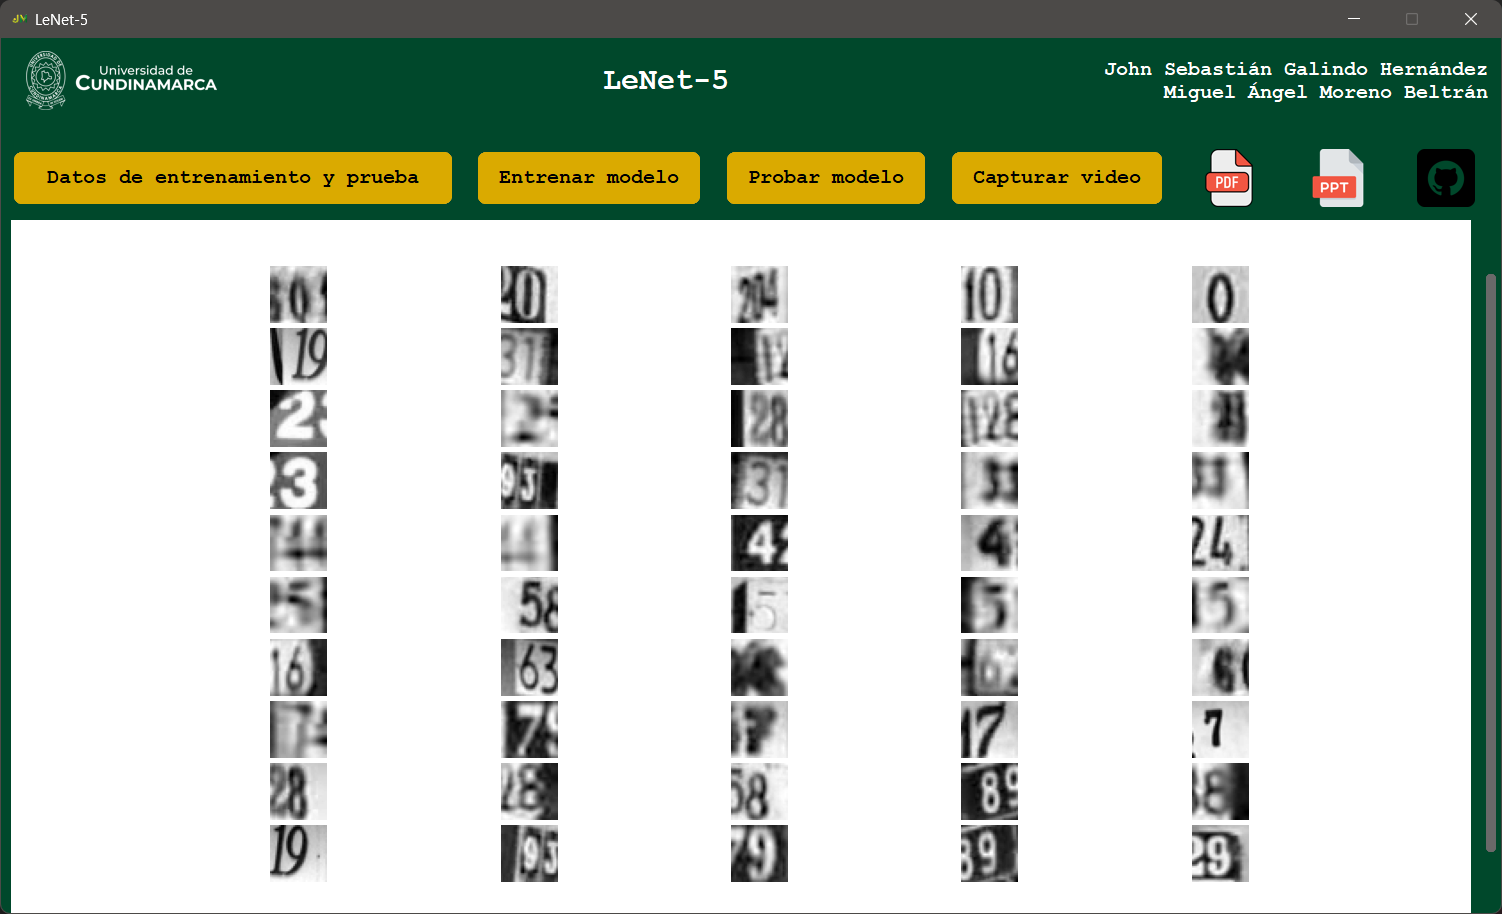
\includegraphics[width=\linewidth]{src/figures/info_function.png}
        \caption{Datos de Entrenamiento}
        \label{fig:TrainingData}
    \end{figure}

    \item \textbf{Entrenar la Red:} El usuario puede entrenar la red neuronal LeNet 5 con los datos de
    MNIST o SVHN, después de que el usuario seleccione la base de datos, la red carga los datos y 
    comienza el entrenamiento, el entrenamiento se puede ver por consola y la arquitectura de la red
    junto con los pesos resultantes para los kernels de la primera y segunda capa convolucional.

    \begin{figure}[htbp]
        \centering
        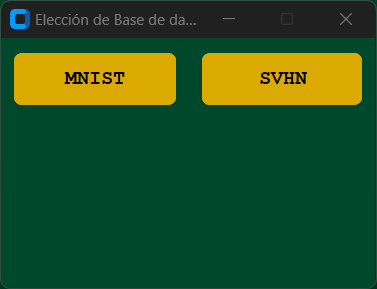
\includegraphics[width=0.6\linewidth]{src/figures/eleccion_bd.png}
        \caption{Selección de la Base de Datos} 
        \label{fig:bd_selection} 
    \end{figure}

    \begin{figure}[H]
        \centering
        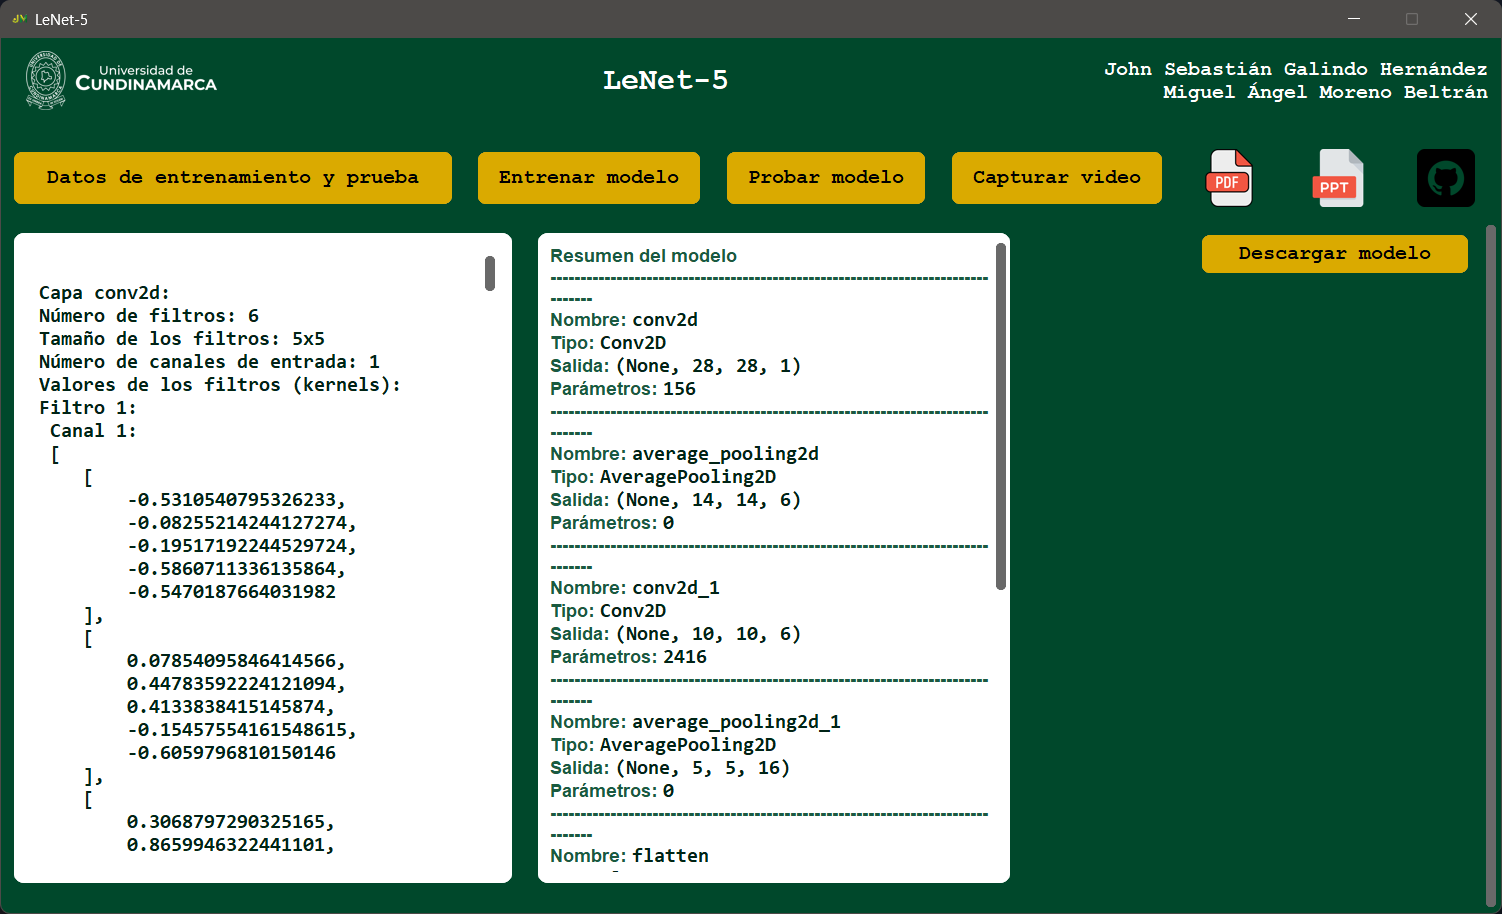
\includegraphics[width=\linewidth]{src/figures/datos_entrenamiento.png}
        \caption{Entrenamiento de la Red}
        \label{fig:data_training}
    \end{figure}

    \item \textbf{Probar la Red:} El usuario puede probar la red neuronal LeNet 5 con la imagen que el 
    seleccione desde el explorador de archivos, la red carga la imagen y la procesa para adecuarla a la red
    redimensionando la imagen y convirtiendola a escala de grises, después de esto la red realiza la predicción
    y se muestra tanto la imagen procesada como la predicción y las probabilidades de cada clase.

    \begin{figure}[H]
        \centering
        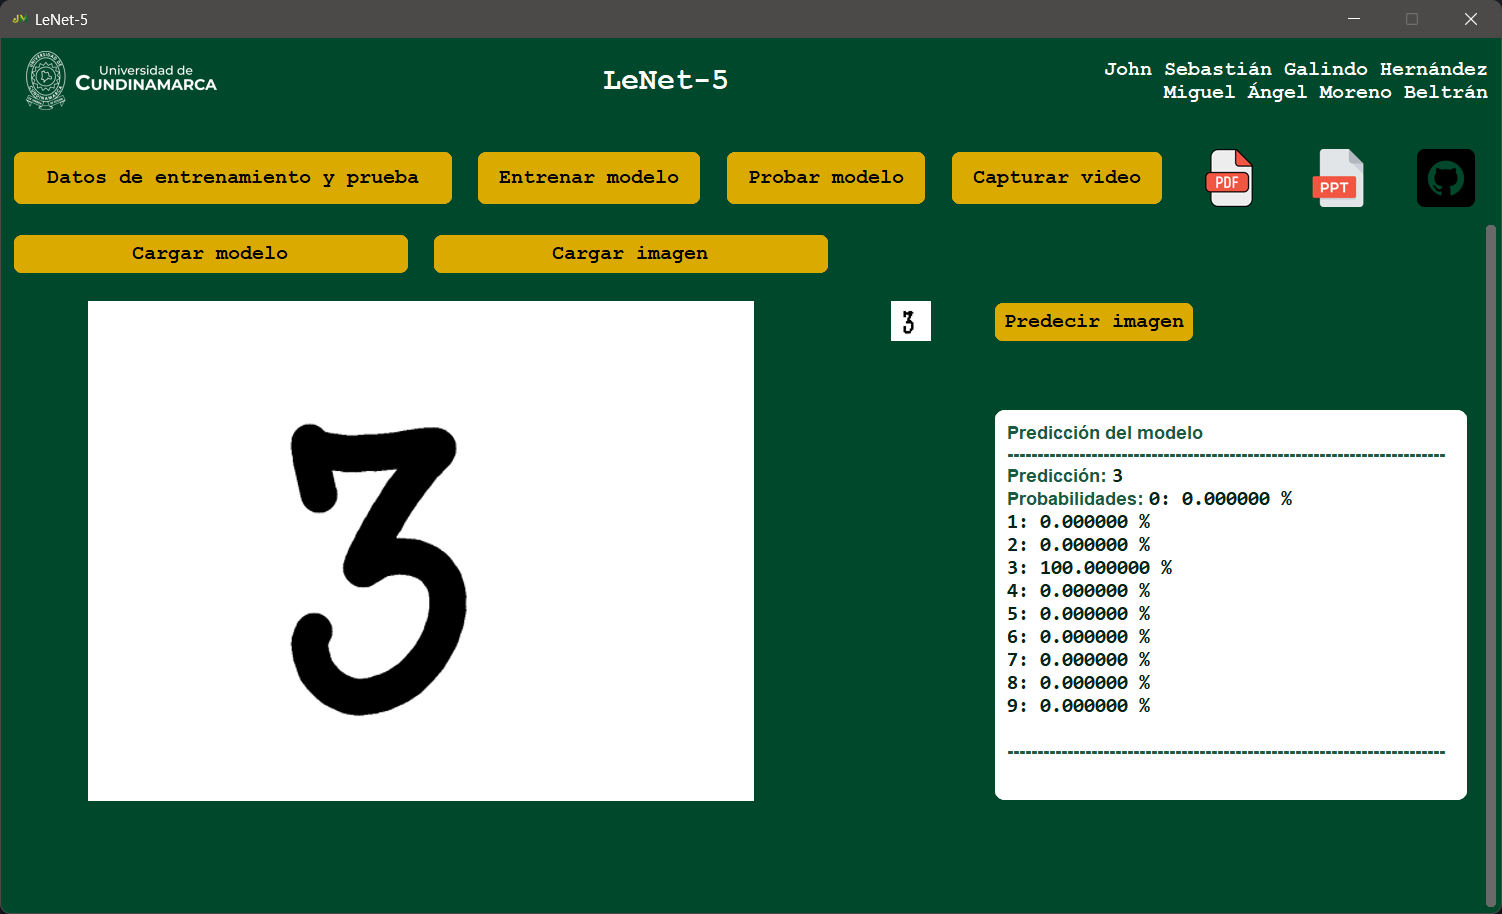
\includegraphics[width=\linewidth]{src/figures/prediccion_funcion.png}
        \caption{Sección de prueba de la Red}
        \label{fig:Test}
    \end{figure}

    \item \textbf{Capturar video:} El usuario puede capturar un video con la cámara de su computadora, la
    cámara que tenga conectada o la camara por IP, ya que esta se especifica mediante un texto ingresado en la GUI.
    una vez se hace conexion con la camara especificada se puede capturar el video y la red realiza la predicción
    de los números que se encuentren en el en tiempo real.

    \begin{figure}[H]
        \centering
        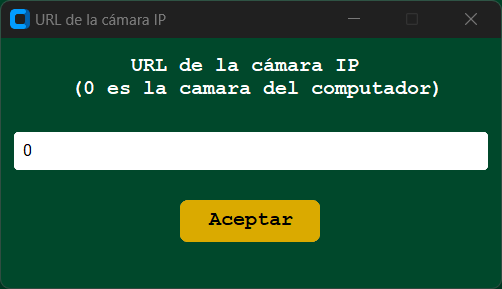
\includegraphics[width=\linewidth]{src/figures/url_camera.png}
        \caption{Sección de captura de Video}
        \label{fig:url_camera}
    \end{figure}

    \begin{figure}[H]
        \centering
        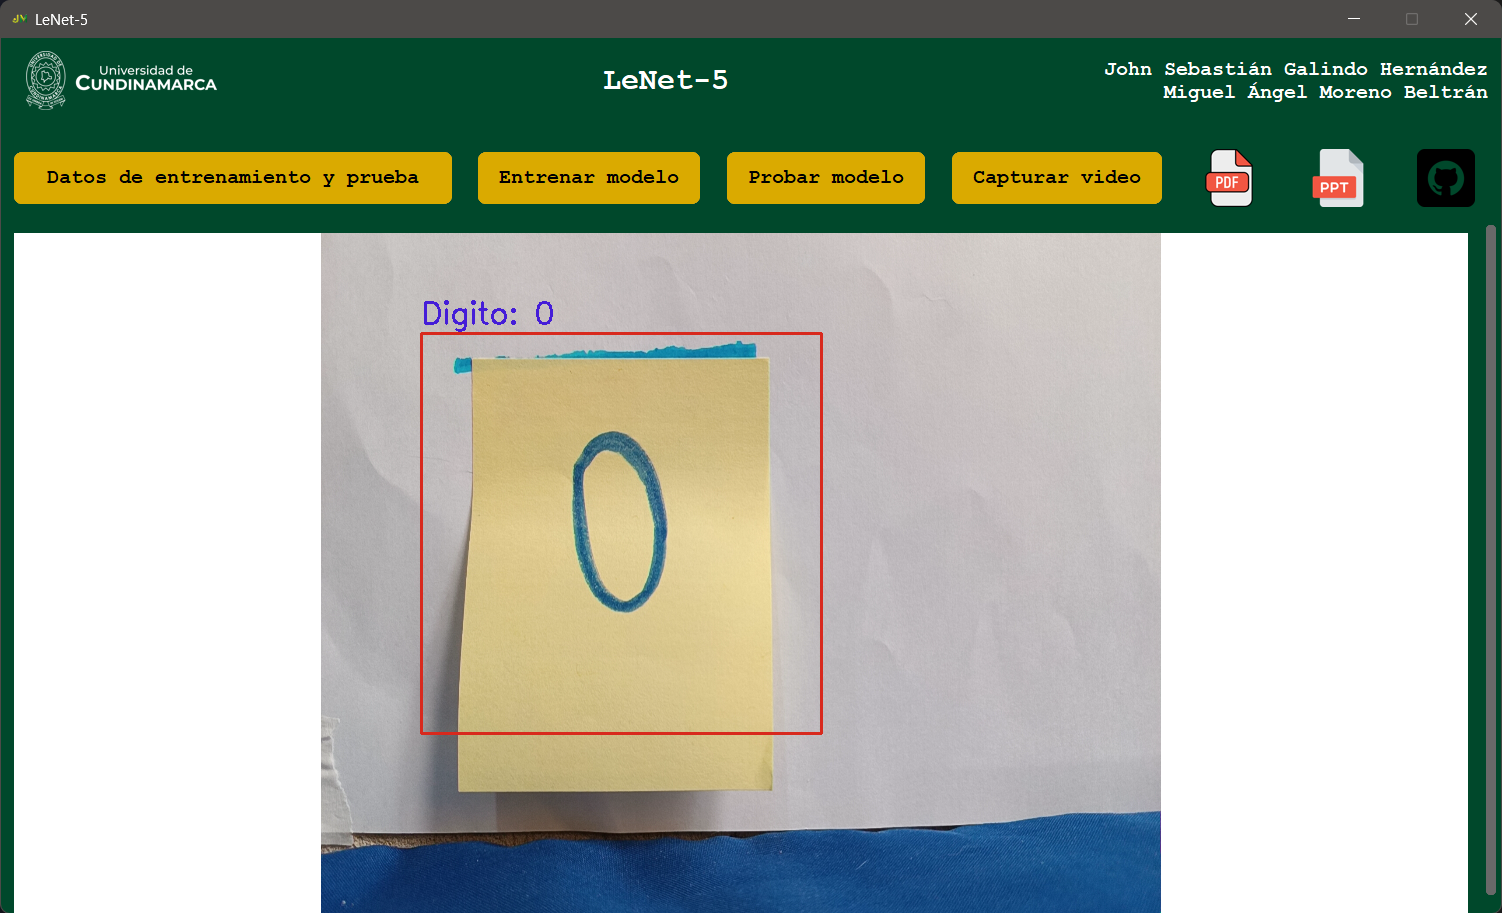
\includegraphics[width=\linewidth]{src/figures/real_test_image_0.png}
        \caption{Captura de Video}
        \label{fig:VideoCapture}
    \end{figure}
\end{itemize}

\subsection{Resultados del entrenamiento de la Red LeNet 5}
Para el entrenamiento de la red LeNet 5 se utilizo la base de datos de MNIST y SVHN, en ambos casos se
utilizó el optimizador adam y la función de activación ReLU para las capas ocultas, después de que 
se realizó el entrenamiento se obtuvieron los siguientes resultados:

\begin{figure}[htbp]
    \centering
    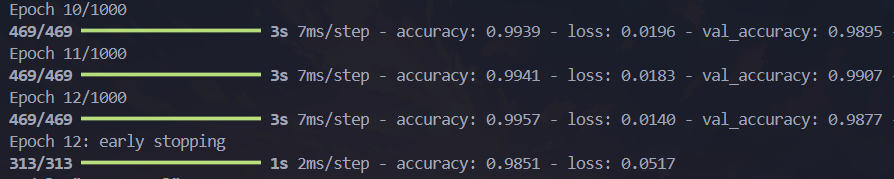
\includegraphics[width=1.1\linewidth]{src/figures/mnist_training.png}
    \caption{Resultados del entrenamiento con MNIST}
    \label{fig:MNISTResults}
\end{figure}

\begin{figure}[htbp]
    \centering
    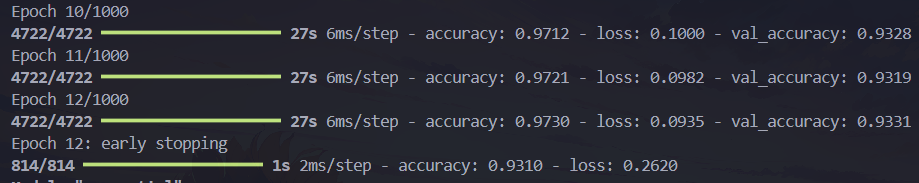
\includegraphics[width=1.1\linewidth]{src/figures/lenet_training.png}
    \caption{Resultados del entrenamiento con SVHN}
    \label{fig:SVHNResults}
\end{figure}

Como se puede comprobar, los resultados obtenidos en el entrenamiento de la red LeNet 5 con la base de datos
MNIST y SVHN son muy buenos, ya que en ambos casos se obtuvo una precisión por encima del 90\% en el conjunto
sin embargo al tener menos datos MNIST y al necesitar que las imagenes esten con la escala de grises invertida
se obtiene una menor tasa de acierto en la predicción de los números que no estén lo suficientemente contrastados
con el fondo. Es por este motivo, que se recomienda el uso de la base de datos SVHN para el entrenamiento de la red
ya que se han realizado pruebas con la base de datos y se ha obtenido una precisión muy alta con imagenes con un 
ruido muy alto.

Por otra parte, se realiza la comparación entre el entrenamiento dado en la figura \ref{fig:SVHNResults} y
los mismos datos con las funciones de activación (Tangente Híperbolica) y el optimizador de gradiente descendiente los
cuales se usaban originalmente en la red LeNet 5, los resultados obtenidos para la prueba original son los siguientes:

\begin{figure}[htbp]
    \centering
    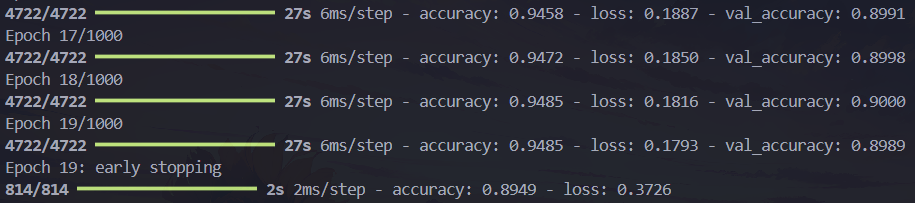
\includegraphics[width=\linewidth]{src/figures/original_info_training.png}
    \caption{Resultados del entrenamiento con SVHN}
    \label{fig:SVHNResultsOriginal}
\end{figure}

Como se puede observar, los resultados obtenidos con la función de activación ReLU y el optimizador Adam son
mejores que los obtenidos con la función de activación Tangente Híperbolica y el optimizador de gradiente descendiente,
ya que no solo alcanza una precisión mayor, sino que también el tiempo de entrenamiento es menor, para el entrenamiento
con los hiperparametros orginales el tiempo total fue de 9 minutos y 30 segundos logrando una precisión en el conjunto de
prueba de 89.5\% mientras que con los nuevos hiperparametros (ReLU y Adam) el tiempo total fue de 5 minutos y 30 segundos 
logrando una precisión en el conjunto de prueba de 93.1\%.

\subsection{Resultados de la Predicción de la Red LeNet 5}

Para la predicción de la red LeNet 5 se utilizo la base de datos de MNIST y SVHN, en ambos casos se tuvieron
algunos errores cuando los datos no estaban tenian muchas irregularidades o cuando su posicion no era la adecuada,
aún asi, con los datos de MNIST se obtuvo un grande error con al probar con imagenes de numeros que tienen estilos 
de caligrafia. Por otro lado, con la base de datos SVHN se obtuvieron resultados muy buenos, tanto para caligrafias
de computadora como para datos escritos a mano e incluso para imagenes de numeros en pinturas o con texturas muy
ruidosas.

Uno de los ejemplos de un resultado presentado trabajando con el modelo entrenado con la base de datos SVHN es el
siguiente:

\begin{figure}[htbp]
    \centering
    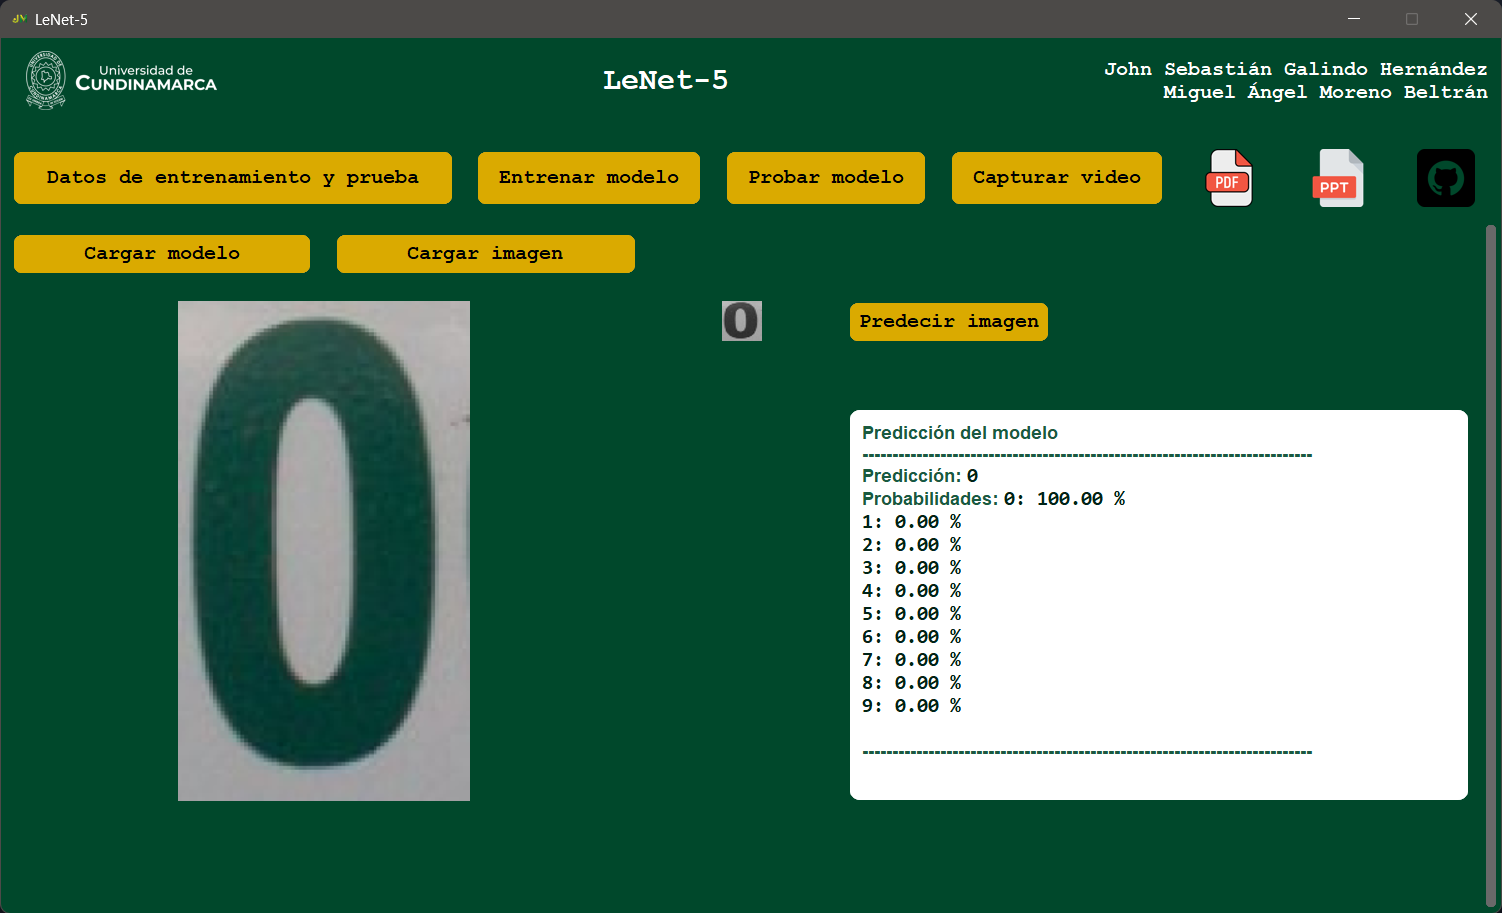
\includegraphics[width=\linewidth]{src/figures/pic_test_image_0.png}
    \caption{Predicción de la Red LeNet 5 para el número 0}
    \label{fig:Prediction_pic_0}
\end{figure}

\begin{figure}[htbp]
    \centering
    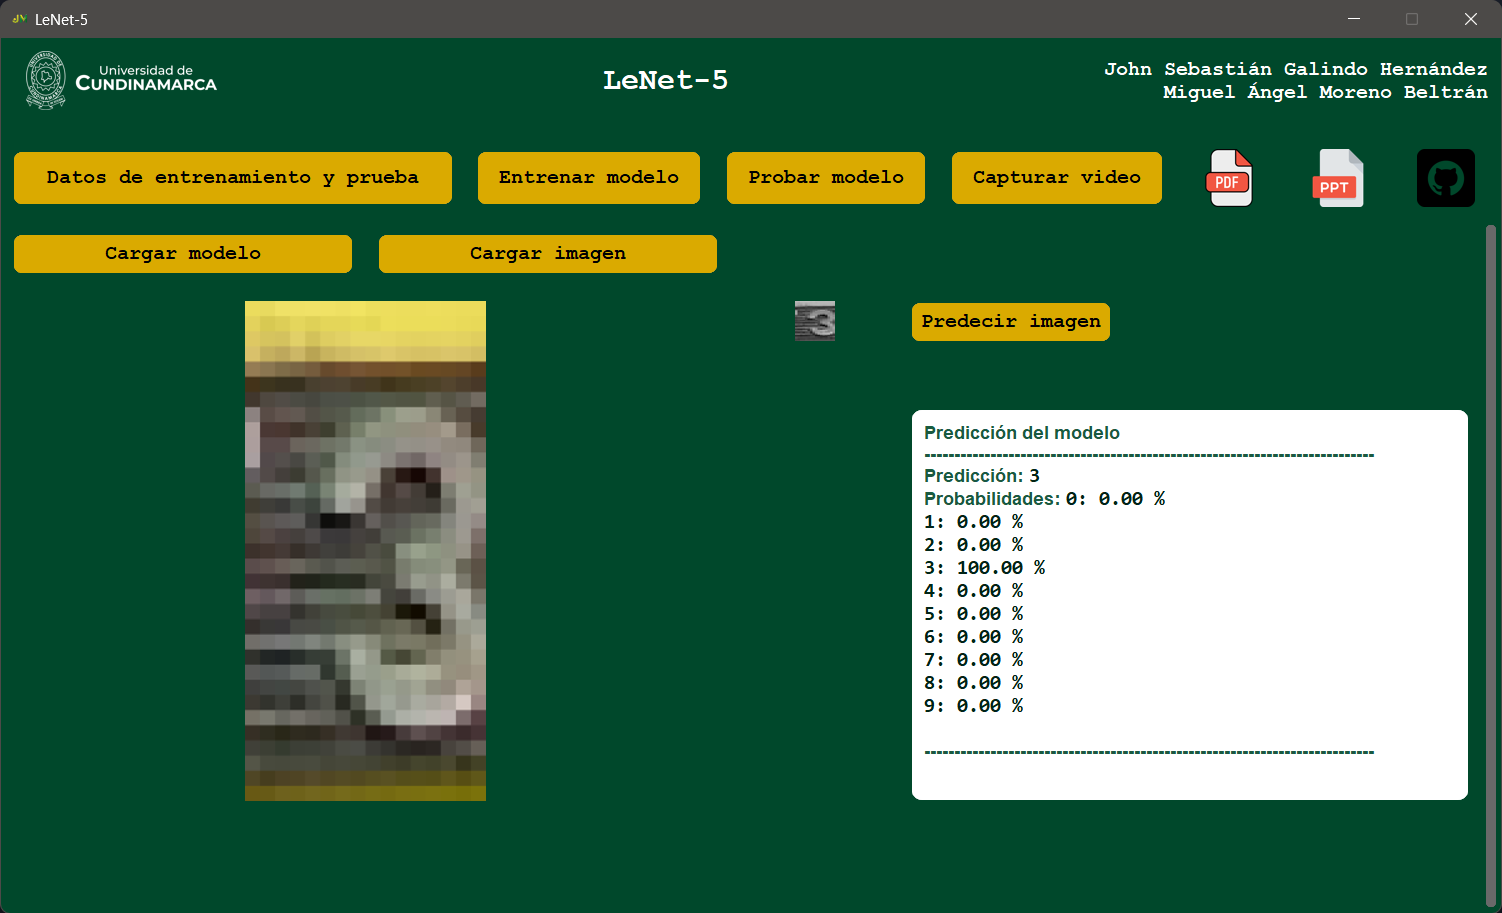
\includegraphics[width=1.05\linewidth]{src/figures/pic_test_image_3.png}
    \caption{Predicción de la Red LeNet 5 para el número 3 con baja resolución}
    \label{fig:Prediction_pic_1}
\end{figure}

Aún cuando hay resultados buenos, el modelo no es perfecto y se puede mejorar, por ejemplo, en la 
siguiente predicción se puede observar que el modelo no es capaz de predecir correctamente el número y 
termina distribuyendo la probabilidad entre varios números lo cual no es habitual en la red LeNet 5.

\begin{figure}[htbp]
    \centering
    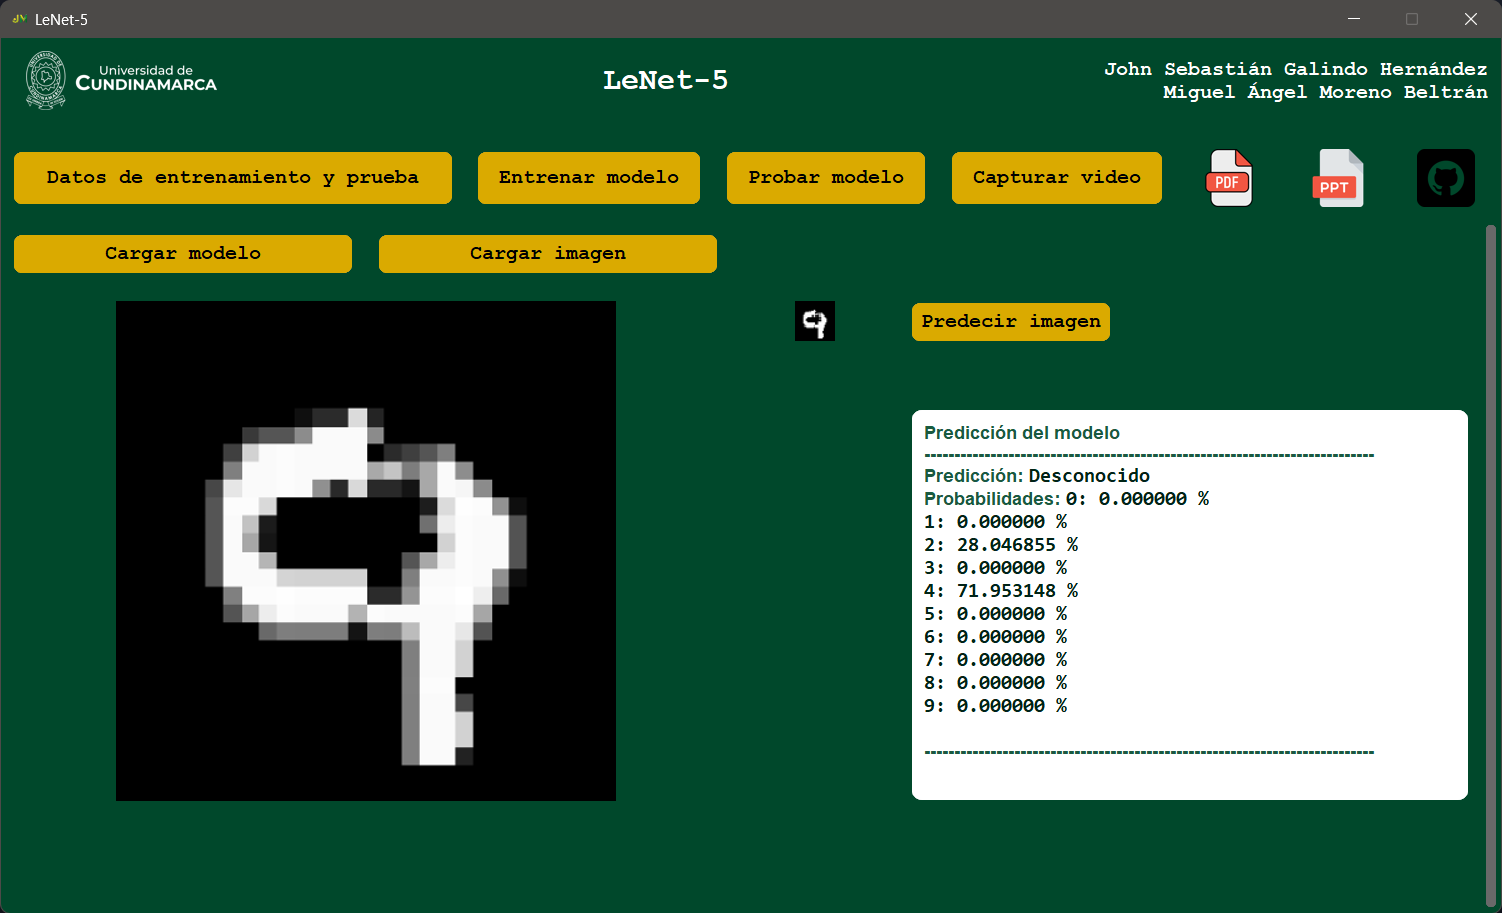
\includegraphics[width=1.05\linewidth]{src/figures/pic_test_image_prob.png}
    \caption{Predicción de la Red LeNet 5 para el número 9}
    \label{fig:Prediction_pic_2}
\end{figure}

todas las imagenes de prueba fueron obtenidas del conjunto de datos Numerical Images encontrado en 
la pagina web de \textbf{Kaggle} \cite{kaggle_data}.

\subsection{Resultados de la Captura de Video}

Para la captura de video se utilizo la cámara de un celular conectado mediante IP con una resolución de 
1080p, en la captura de video se obtuvieron resultados muy buenos pero que eran muy susceptibles a la
posicion del número en el recuadro de información, ya que si el número no estaba centrado o si estaba
muy inclinado la red no era capaz de predecir correctamente el número, sin embargo, los resultados 
en general fueron muy buenos y se obtuvo un resultado correcto en la gran mayoría de los casos.
A continuación se presentan una serie de pruebas realizadas para los numeros desde el 0 hasta el 9.

\begin{figure}[H]
    \centering
    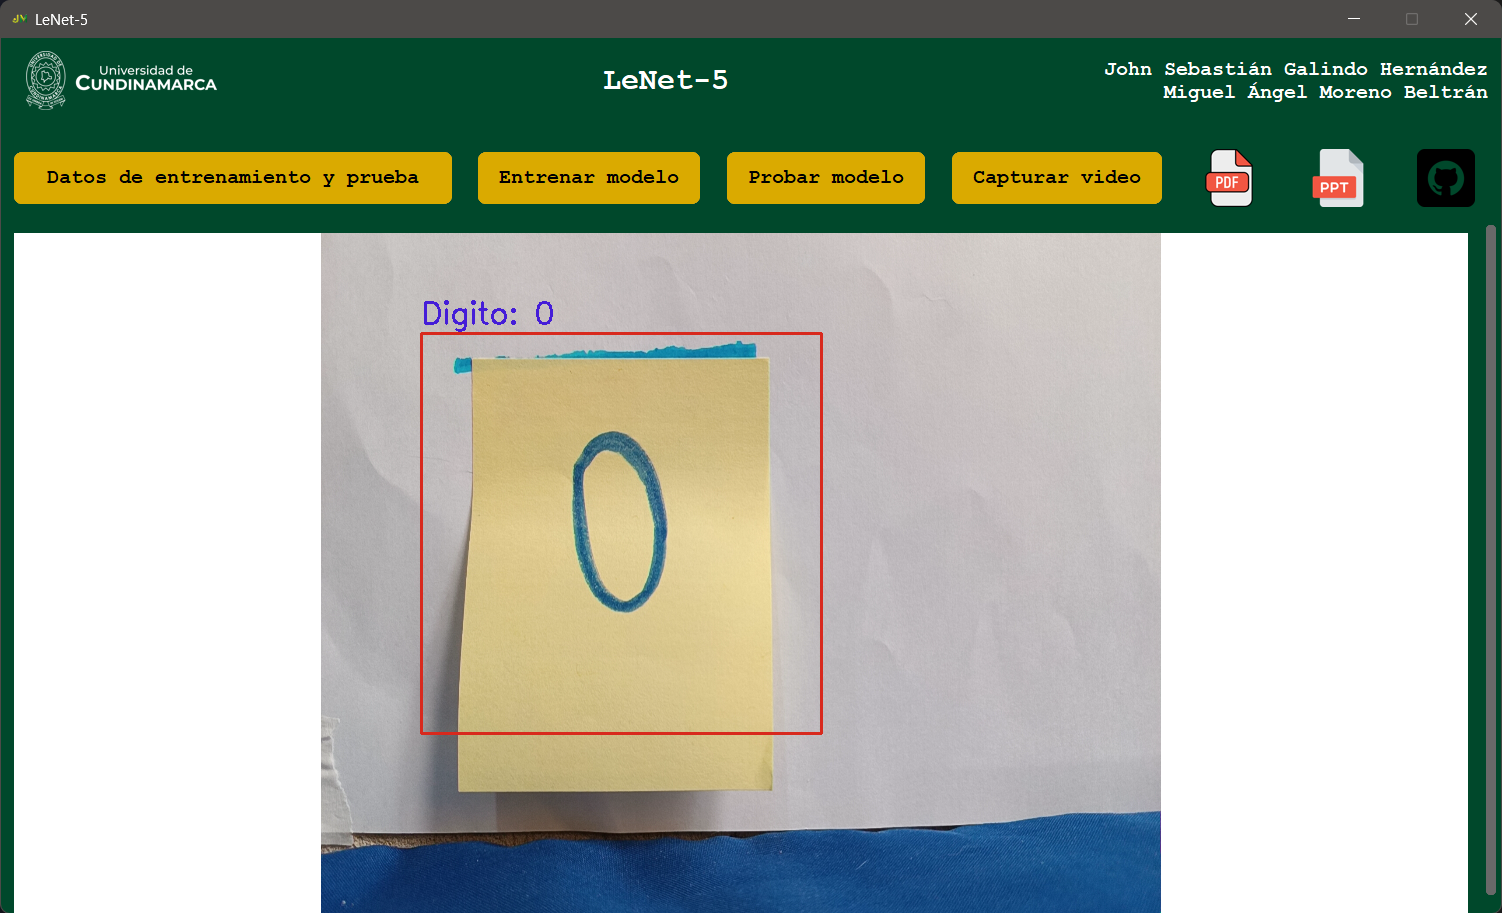
\includegraphics[width=\linewidth]{src/figures/real_test_image_0.png}
    \caption{Predicción en tiempo real de la Red LeNet 5 para el número 0}
    \label{fig:RealTest_0}
\end{figure}

\begin{figure}[H]
    \centering
    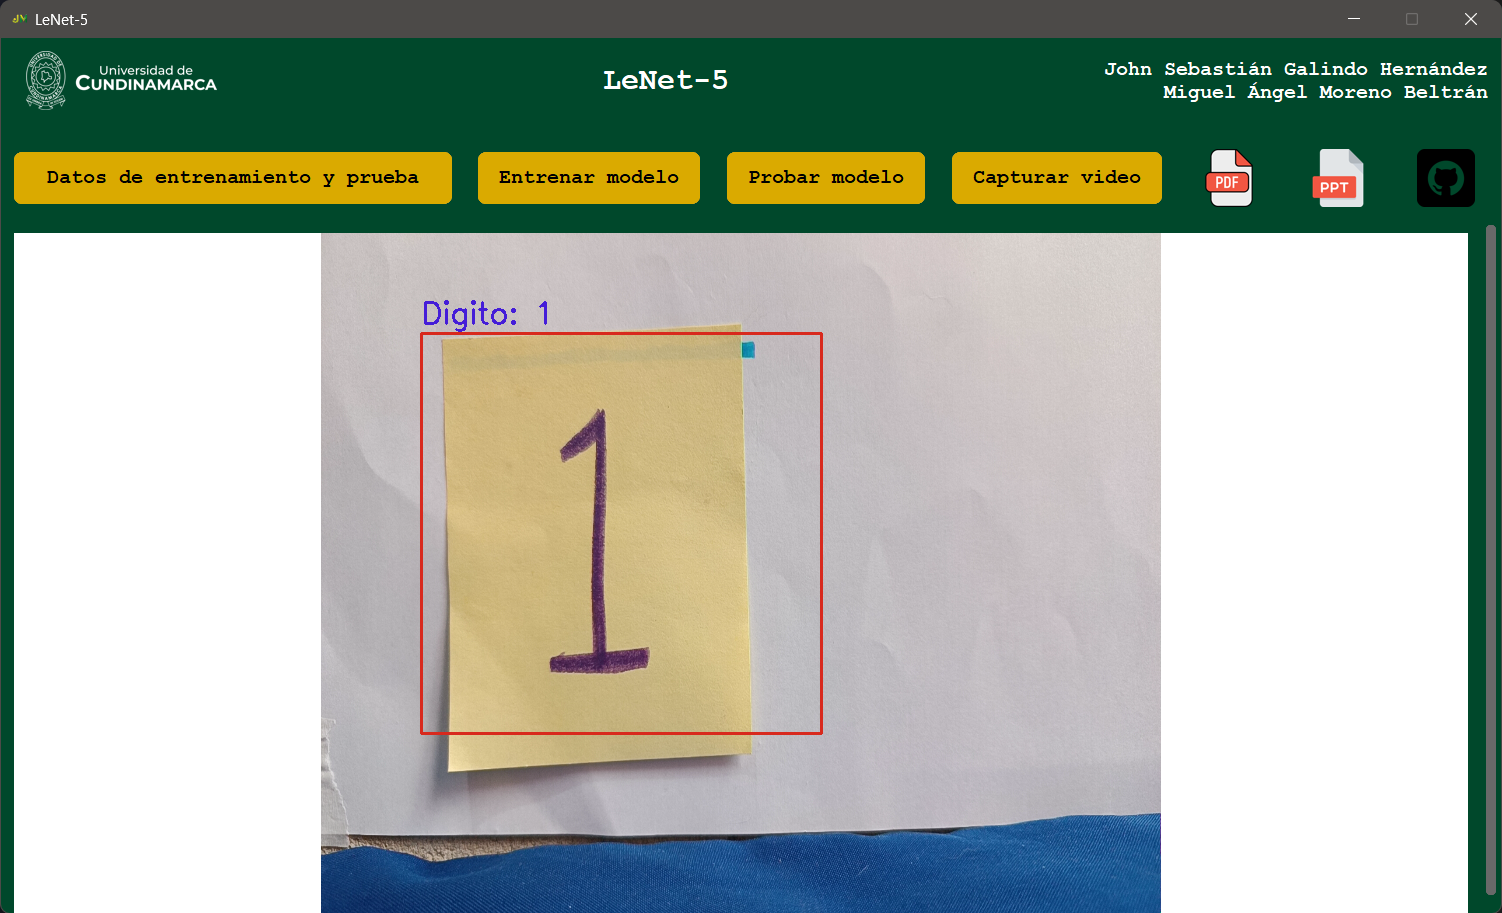
\includegraphics[width=\linewidth]{src/figures/real_test_image_1.png}
    \caption{Predicción en tiempo real de la Red LeNet 5 para el número 1}
    \label{fig:RealTest_1}
\end{figure}

\begin{figure}[H]
    \centering
    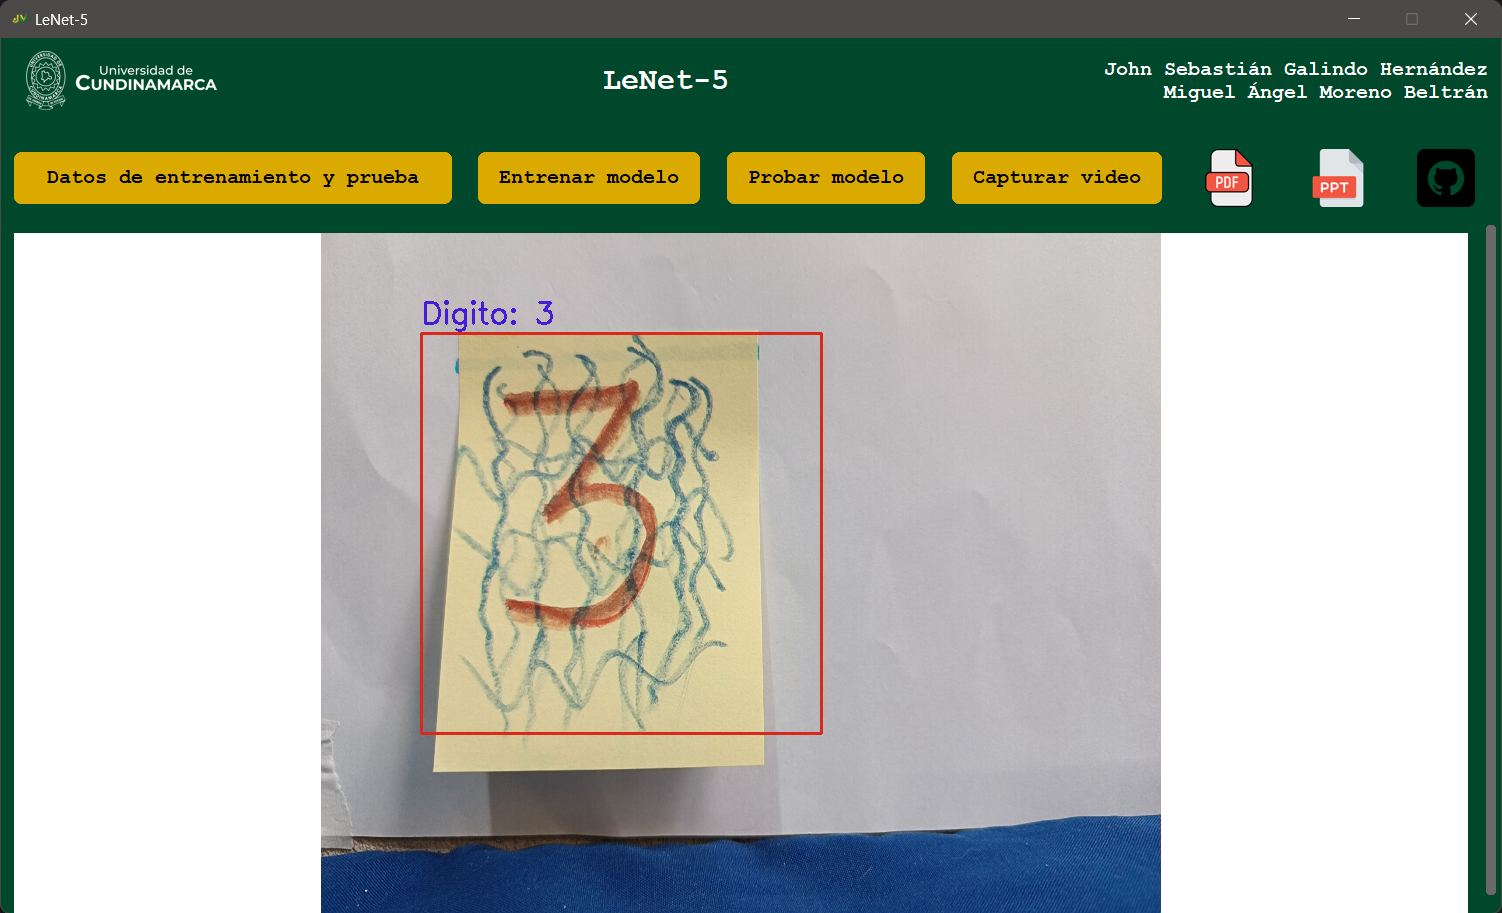
\includegraphics[width=\linewidth]{src/figures/real_test_image_3.png}
    \caption{Predicción en tiempo real de la Red LeNet 5 para el número 3}
    \label{fig:RealTest_3}
\end{figure}

\begin{figure}[H]
    \centering
    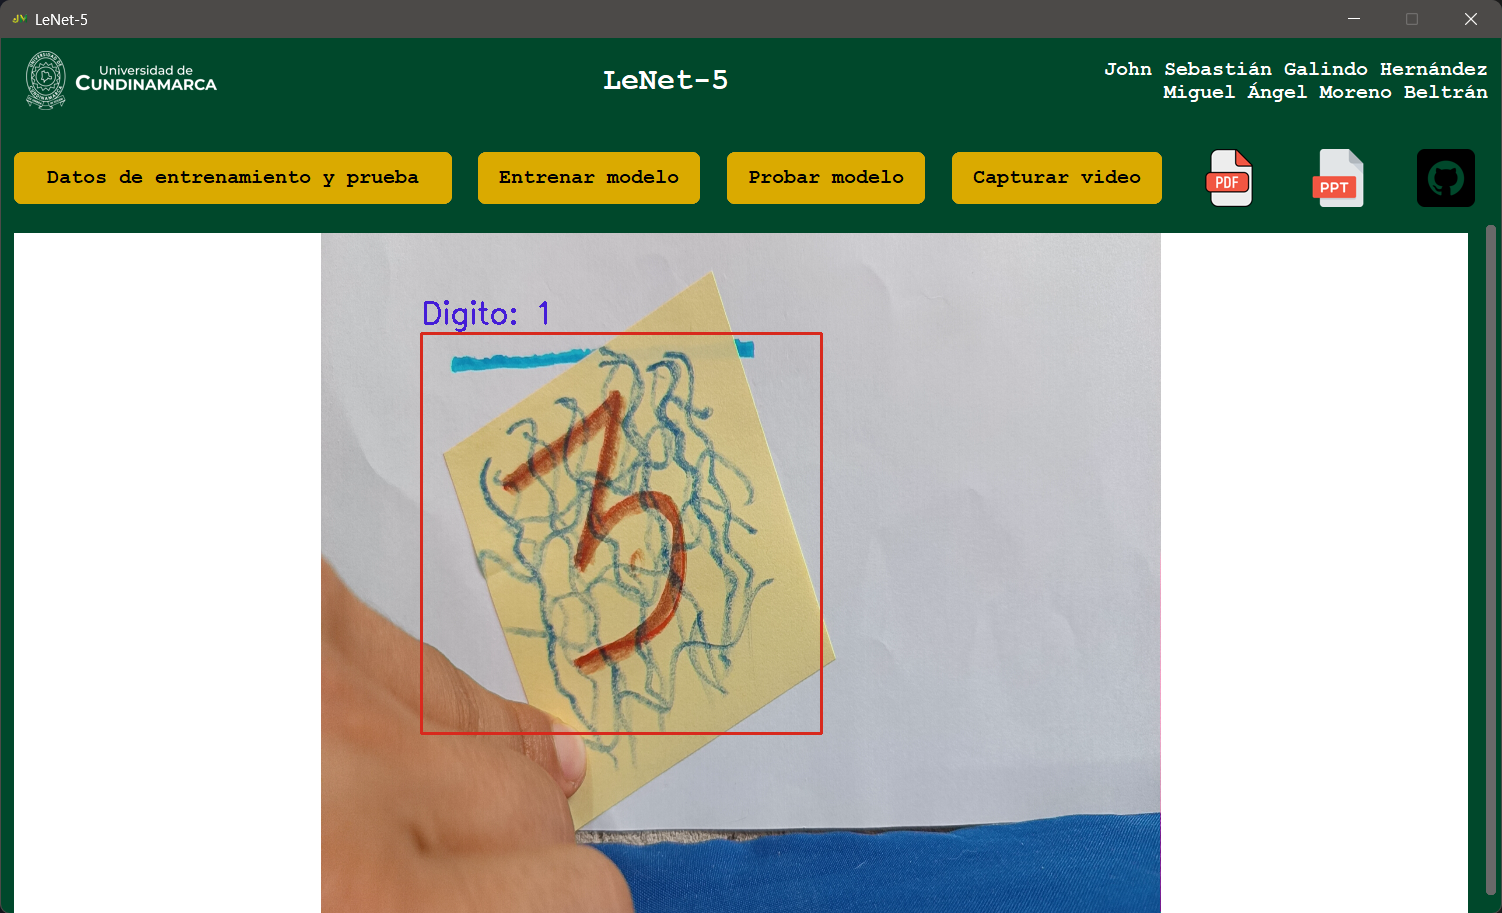
\includegraphics[width=\linewidth]{src/figures/real_test_image_3-2.png}
    \caption{Predicción en tiempo real de la Red LeNet 5 para el número 3 inclinado}
    \label{fig:RealTest_3_2}
\end{figure}

\begin{figure}[H]
    \centering
    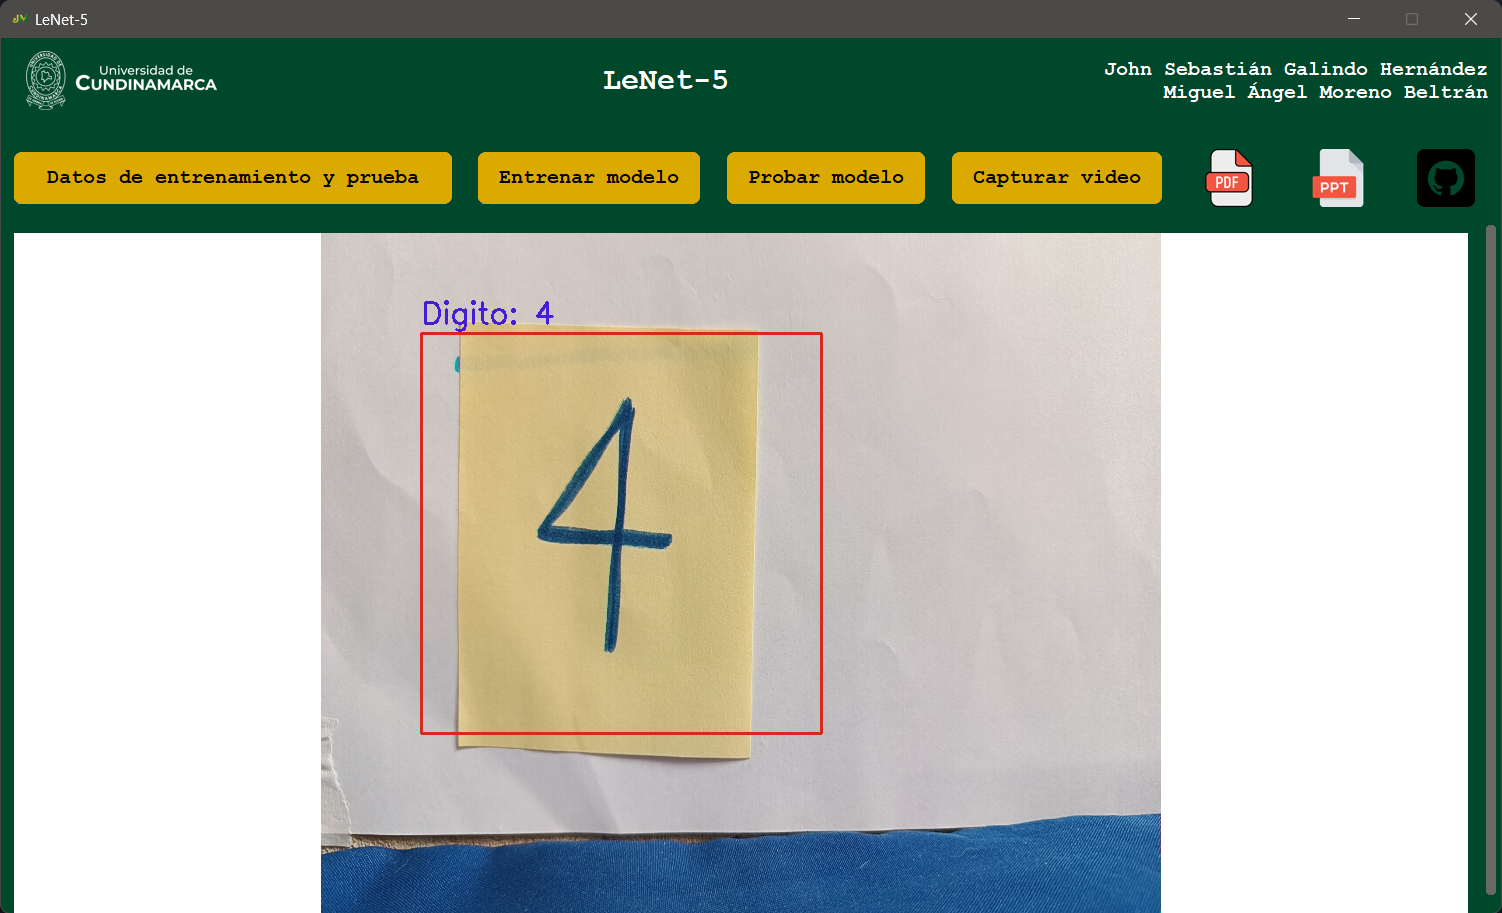
\includegraphics[width=\linewidth]{src/figures/real_test_image_4.png}
    \caption{Predicción en tiempo real de la Red LeNet 5 para el número 4}
    \label{fig:RealTest_4}
\end{figure}

\begin{figure}[H]
    \centering
    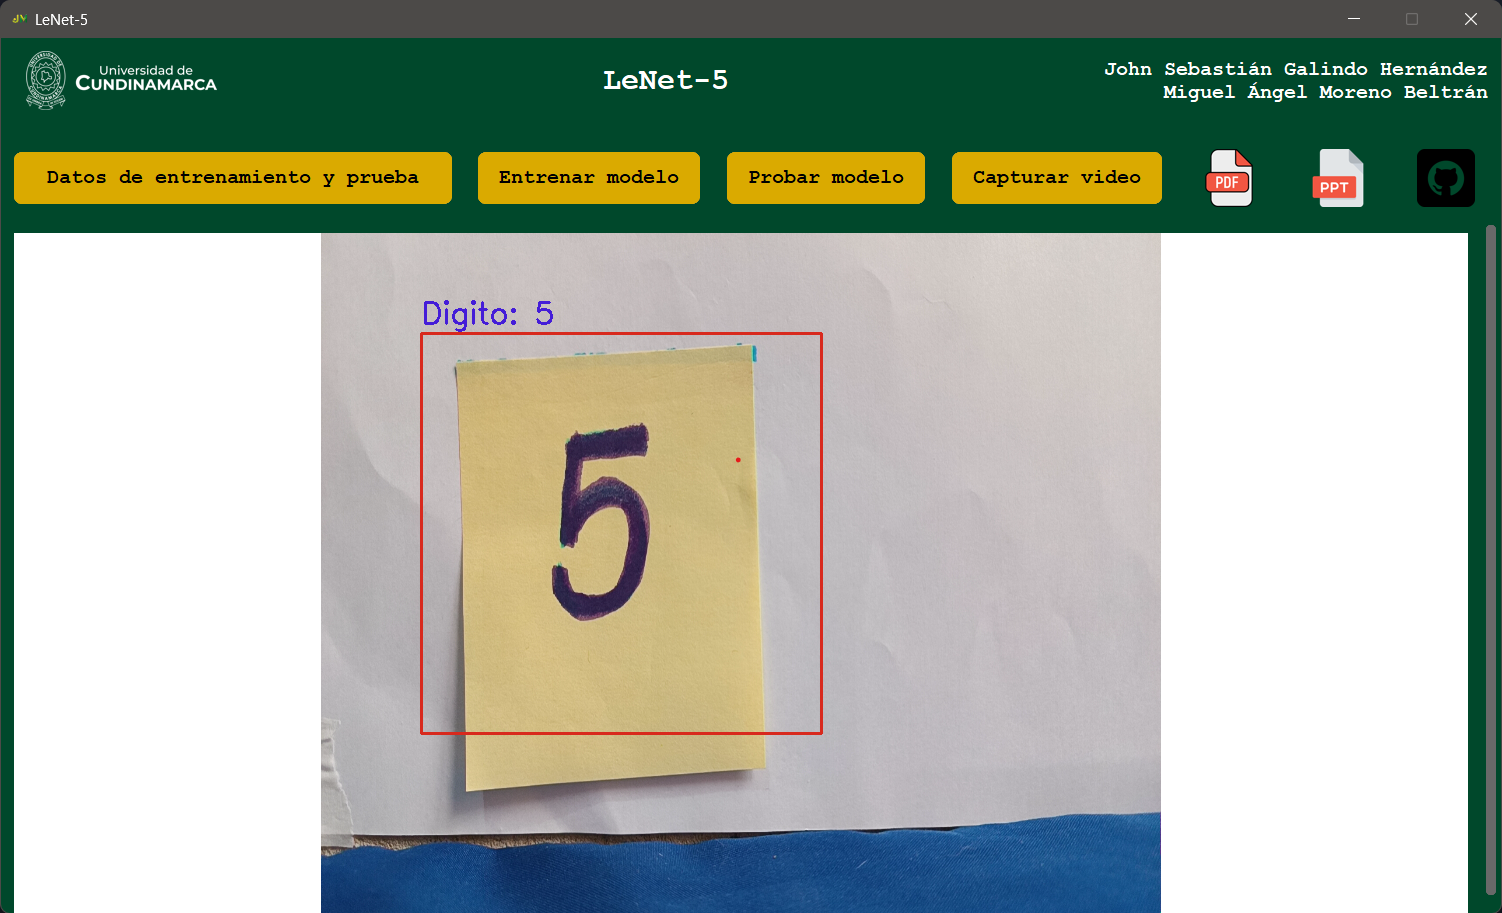
\includegraphics[width=\linewidth]{src/figures/real_test_image_5.png}
    \caption{Predicción en tiempo real de la Red LeNet 5 para el número 5}
    \label{fig:RealTest_5}
\end{figure}

\begin{figure}[H]
    \centering
    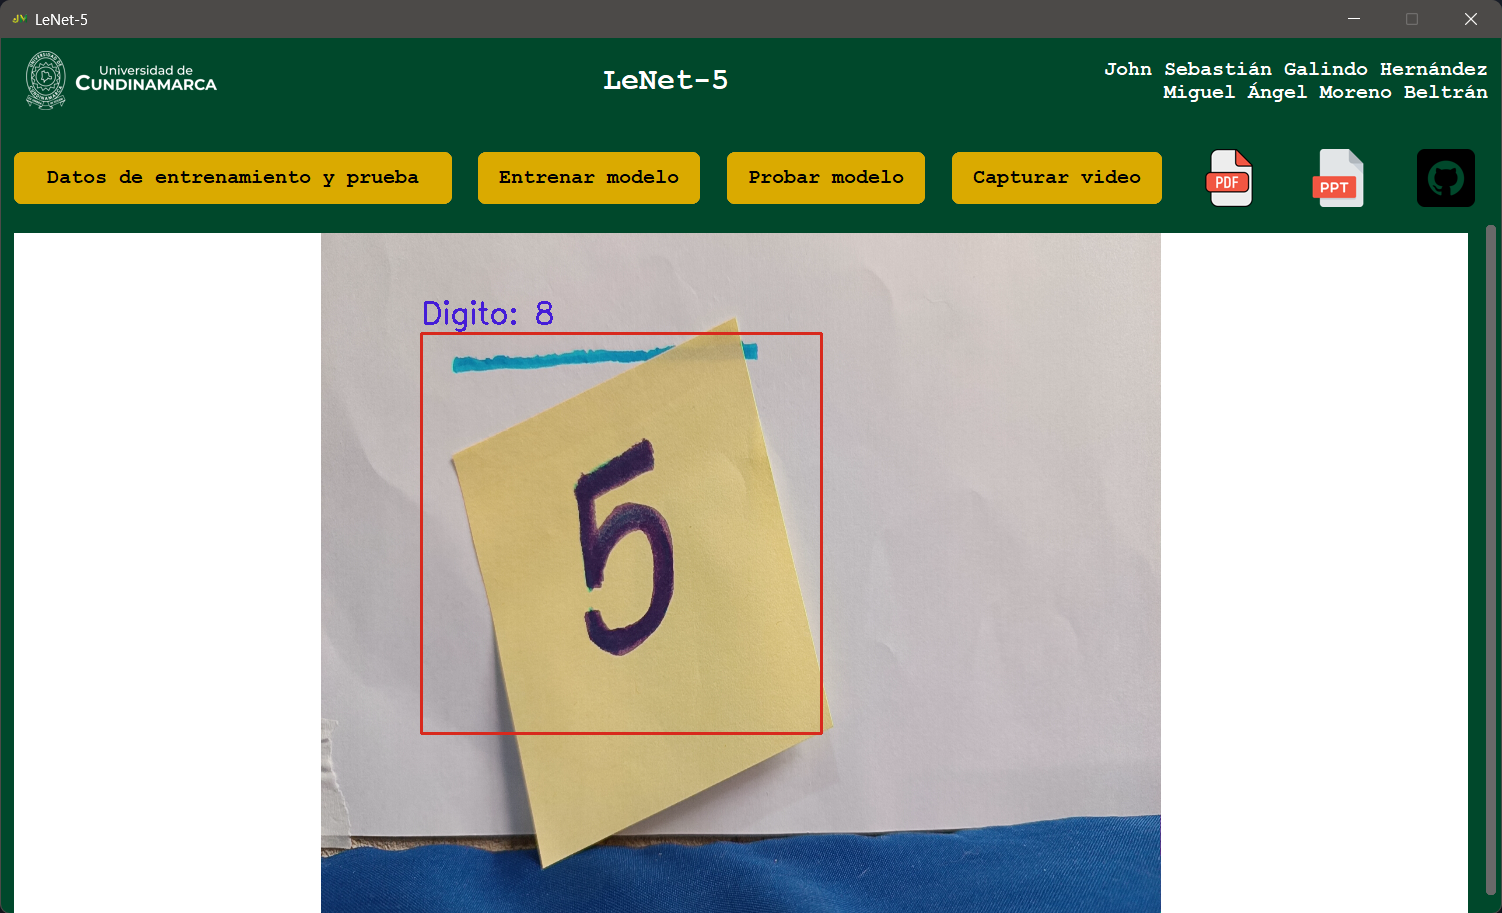
\includegraphics[width=\linewidth]{src/figures/real_test_image_5-2.png}
    \caption{Predicción en tiempo real de la Red LeNet 5 para el número 5 inclinado}
    \label{fig:RealTest_5_2}
\end{figure}

\begin{figure}[H]
    \centering
    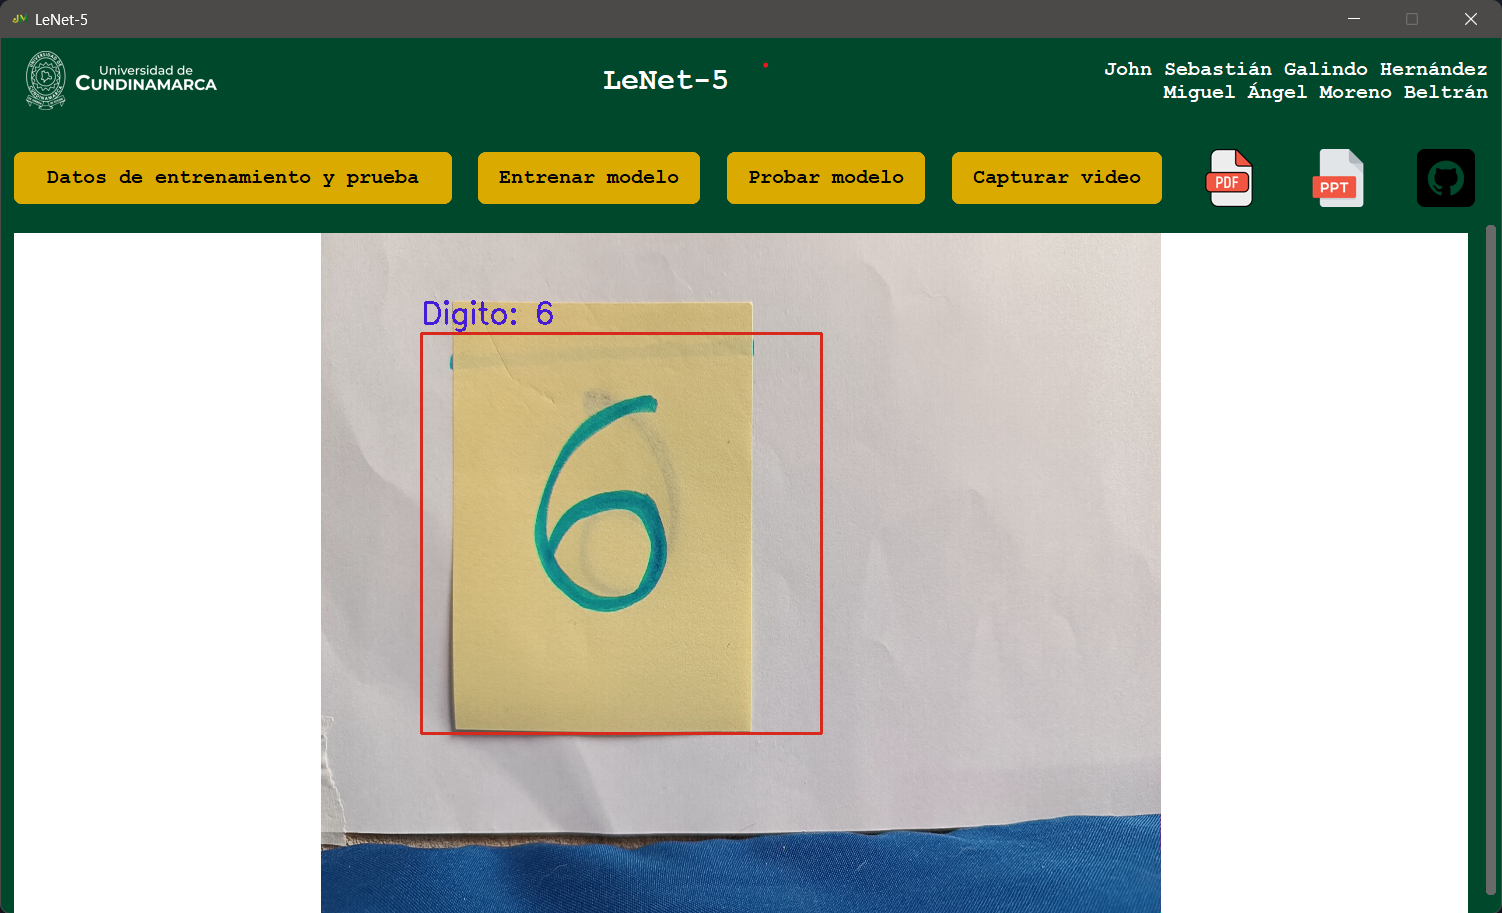
\includegraphics[width=\linewidth]{src/figures/real_test_image_6.png}
    \caption{Predicción en tiempo real de la Red LeNet 5 para el número 6}
    \label{fig:RealTest_6}
\end{figure}

\begin{figure}[H]
    \centering
    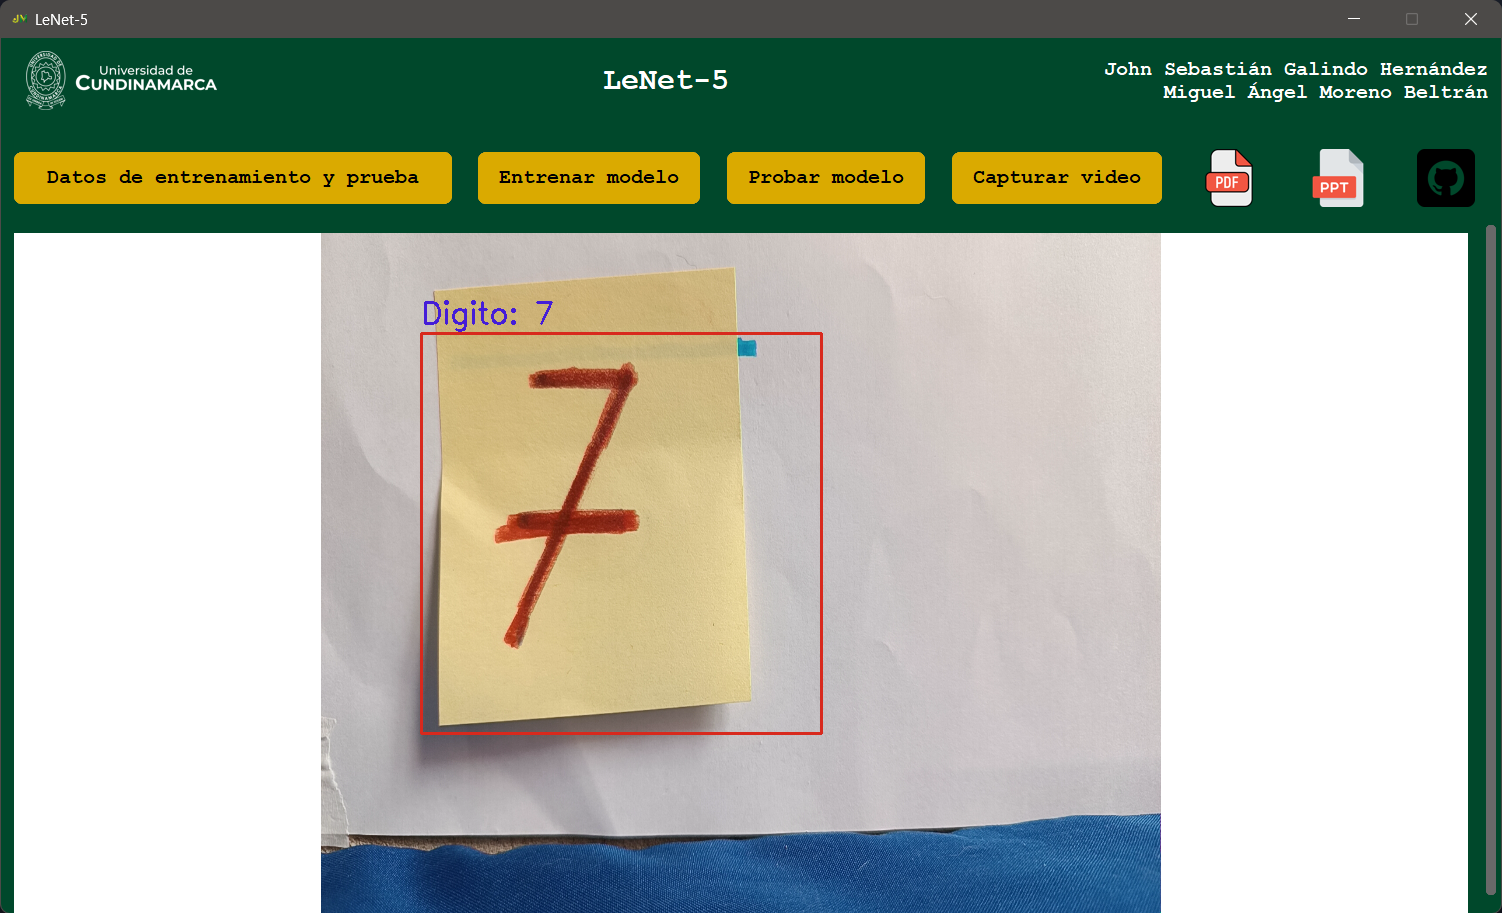
\includegraphics[width=\linewidth]{src/figures/real_test_image_7.png}
    \caption{Predicción en tiempo real de la Red LeNet 5 para el número 7}
    \label{fig:RealTest_7}
\end{figure}

\begin{figure}[H]
    \centering
    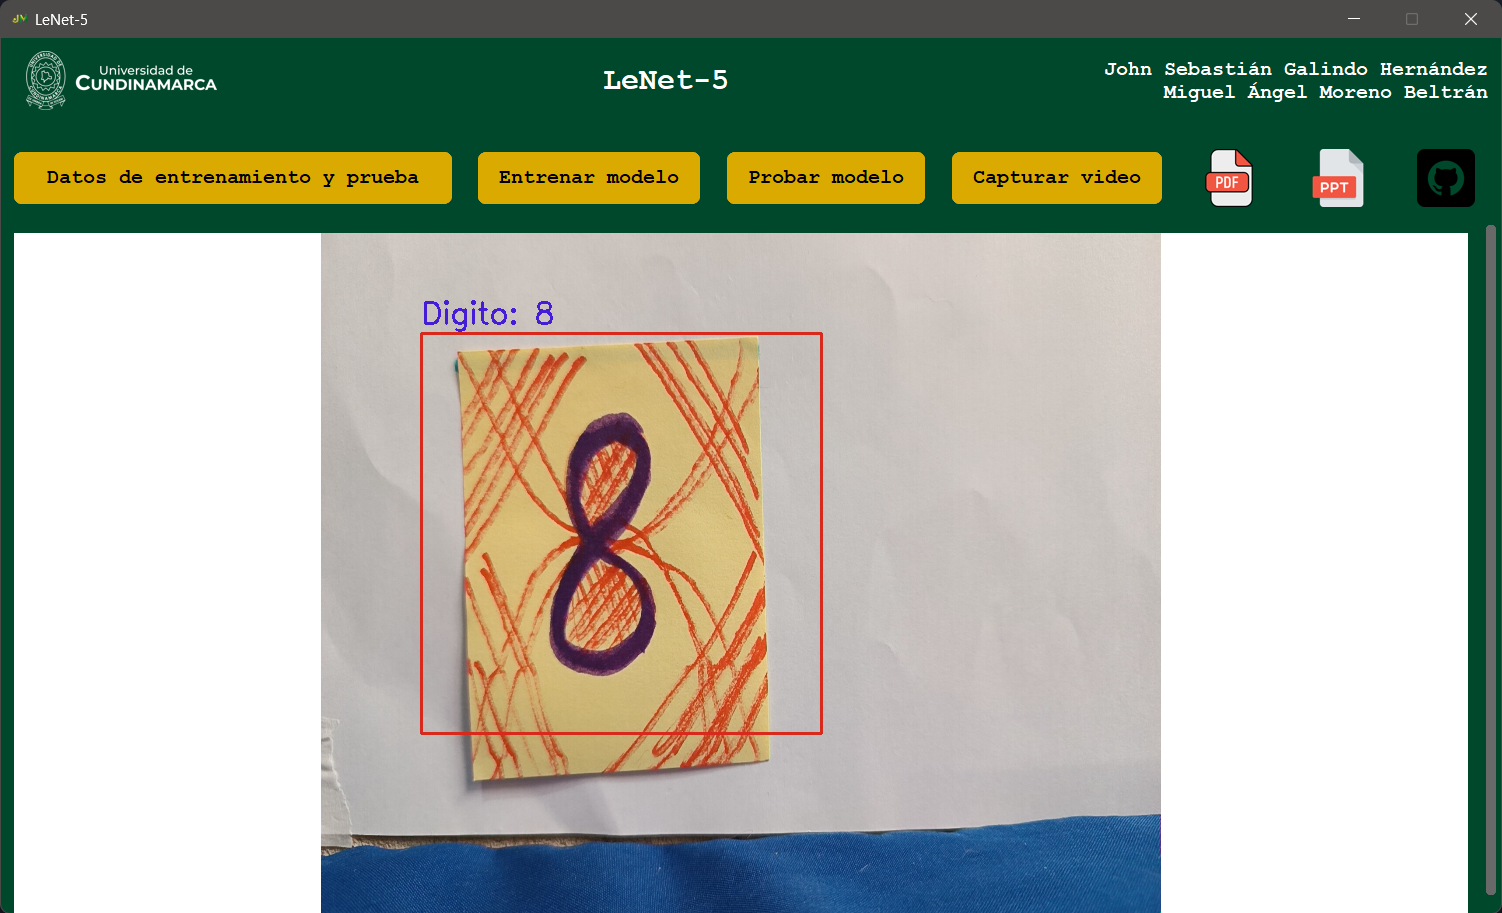
\includegraphics[width=\linewidth]{src/figures/real_test_image_8.png}
    \caption{Predicción en tiempo real de la Red LeNet 5 para el número 8}
    \label{fig:RealTest_8}
\end{figure}

\begin{figure}[H]
    \centering
    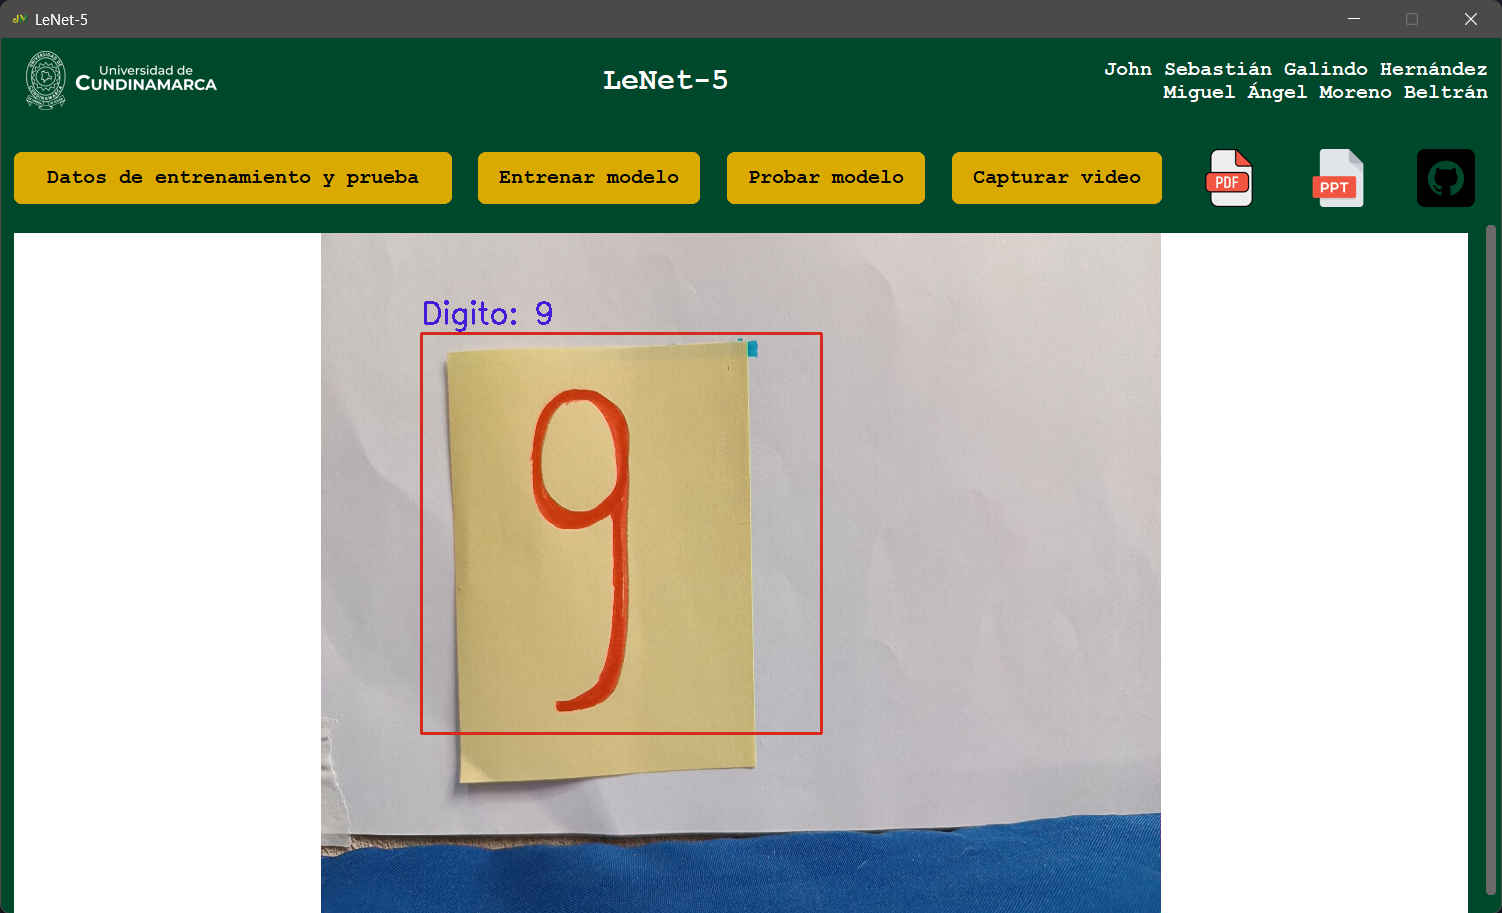
\includegraphics[width=\linewidth]{src/figures/real_test_image_9.png}
    \caption{Predicción en tiempo real de la Red LeNet 5 para el número 9}
    \label{fig:RealTest_9}
\end{figure}

Como se puede ver en las imagenes, se implemento una region de interés (ROI) para que la red solo procese
la parte de la imagen que contiene el número, esto se hizo para mejorar la predicción de la red y para que
la red no se vea afectada por el ruido de la imagen. Por otro lado, se corrobora que ni el ruido ni el color
del número afectan la predicción de la red, ya que se realizaron pruebas con números de diferentes colores y
con números con rayones y la red fue capaz de predecir correctamente el número en la gran mayoría de los casos; 
sin embargo, la red no es perfecta y en algunos casos no es capaz de predecir correctamente el número, sobre todo
cuando el número no esta centrado o cuando el número esta muy inclinado hacia alguno de sus lados, lo que demuestra
que los filtros de la red aprendieron a identificar patrones en base a la posición del número en la imagen, lo cual
cobra sentido al saber que debe diferenciar entre formas similares pero en diferente posicion como las del 6 y el 9.
\section{Conclusiones}

\subsection{John Sebastián Galindo Hernández}
La red neuronal LeNet es un paso gigante de las redes neuronales artificiales 
a las redes neuronales convolucionales, ya que estas últimas son capaces de
reconocer patrones en imágenes, lo cual es una tarea muy compleja y más aún
cuando se tienen muchas categorías a clasificar. La red LeNet es un ejemplo de
una CNN implementada con el objetivo de mantener una generalización en el 
entrenamiento mientras se intenta reducir la información de las imágenes 
originales solo a los patrones más importantes, esto se logra mediante las 
capas de su arquitectura. Adentrandose en la opinion sobre como predice la red
LeNet, se puede decir que es muy buena, ya que en la mayoría de los casos
predice correctamente la categoría de la imagen, sin embargo, en algunos casos
que parecen sencillos para un humano, la red falla, esto se puede deber a que 
los datos de entrenamiento no son suficientes o algunas imagenes tienen un 
ruido que termina confundiendo a la red. En general, la red LeNet es una
herramienta muy útil para clasificar imágenes, pero se debe tener en cuenta que
al trabajar con imágenes en tiempo real se debe tener presente un estandar en
posicionamiento, tamaño y color de las numeros en las imágenes para que la red pueda
clasificar correctamente. Por último, LeNet es una red que obtiene muy bien las 
características y patrones de los datos de entrada, lo cual la hace maleable para
diferentes casos como el de las señales de trafico, las imagenes de cancer de mama,
las imagenes de letras, números y simbolos del codigo ASCII
o las imagenes de multiples dígitos escritos a mano, en esta ultima, también se 
puede comprender que la red puede ser juntada con otras técnicas que segmenten 
la información en una imagen para separar los dígitos y clasificarlos de manera
independiente dando así una clasificación más precisa y que se pueda volver a 
combinar para obtener el número completo.

\subsection{Miguel Ángel Moreno Beltrán}
La red neuronal convolucional LeNet destaca por su relevancia en entornos actuales, 
gracias a su capacidad para generalizar patrones visuales. 
Aunque es limitada para tareas más complejas, su precisión puede mejorarse mediante técnicas avanzadas, 
como se observó con el desarrollo de LeNet-5 y su versión mejorada Boosted LeNet-4. 
En este laboratorio, el uso de funciones de activación modernas como ReLU y 
el optimizador Adam permitieron alcanzar un rendimiento superior del 93.1\%, 
en comparación con las configuraciones originales. 
Para finalizar, LeNet demuestra un rendimiento altamente competitivo en entornos 
específicos y controlados, como el reconocimiento de números en imágenes, 
manteniéndose como una arquitectura eficaz y adaptable a diversas aplicaciones.


\subsection{Conclusion Final}
LeNet ha demostrado ser una red neuronal convolucional pionera y relevante en el ámbito actual, 
gracias a su capacidad para reconocer patrones visuales y clasificar imágenes de forma precisa. 
La arquitectura de LeNet, especialmente en su versión LeNet-5, 
fue un avance significativo hacia el desarrollo de redes neuronales más complejas y adaptadas a 
tareas de procesamiento de imágenes. Las mejoras, como el Boosted LeNet-4, y el uso de técnicas 
modernas como las funciones de activación ReLU y el optimizador Adam, han mostrado que su rendimiento 
puede alcanzar niveles competitivos, con una precisión superior al 93.1\% en condiciones controladas. 
Aunque limitada para algunas tareas complejas y entornos no controlados, 
LeNet sigue siendo una herramienta útil y adaptable a diversas aplicaciones, 
desde el reconocimiento de números y letras hasta el procesamiento de señales de tráfico y la detección 
de anomalías en imágenes médicas. Su capacidad para extraer y generalizar patrones la convierte 
en una opción ideal para proyectos específicos, donde con el apoyo de técnicas complementarias, 
como la segmentación de imágenes, podría mejorar aún más su precisión y aplicabilidad en la clasificación 
de imágenes complejas y ruidosas.

% Bibliografía
\newpage
\bibliographystyle{IEEEtran}
\bibliography{bibliography/bibliography}

\end{document}
